%!TEX root = ../larxxia.tex


\section{Beautiful properties for symmetric matrices}
\label{sec:sm}
\secttoc

\begin{comment}
\pooliv{\S5.4} \layiv{\S7.1} \holti{\S8.3} \cite[\S10]{Davis99a}
\end{comment}



This section starts by exploring two properties for eigenvalues of general matrices, and then proceeds to the special case of real symmetric  matrices.
Symmetric matrices have the beautifully useful properties of always having real eigenvalues and always having \text{orthogonal eigenvectors.}



\subsection{Matrix powers maintain eigenvectors}
\label{sec:mpmev}

\index{eigenvector|(}
Recall that \cref{sec:im} introduced the \idx{inverse} of a matrix (\cref{def:invertible}).
This first theorem links an eigenvalue of zero to the non-existence of an inverse, and hence links a zero eigenvalue to problematic \idx{linear equation}s.


\begin{theorem} \label{thm:evalinv} 
A \idx{square matrix} is \idx{invertible} \idx{iff} \idx{zero} is \emph{not} an \idx{eigenvalue} of the matrix.
\end{theorem}
\begin{proof} 
From \cref{def:evecval}, zero is an eigenvalue (\(\lambda=0\)) iff \(A\xv=0\xv\) has nonzero solutions~\xv; that is, iff the homogeneous system \(A\xv=\ov\) has nonzero solutions~\xv.
But the Unique Solution \cref{thm:ftim1,thm:ftim2} assure us that this occurs iff matrix~\(A\) is not invertible.
Consequently a matrix is invertible iff zero is not \text{an eigenvalue.}
\end{proof}

\begin{example} 
\begin{itemize}
\item The \(3\times 3\) matrix of \cref{eg:eig3intro,eg:eig3sp,eg:eig3eig,eg:eig3introval} is not invertible as among its eigenvalues of \(0\), \(1\), and~\(3\) it has zero as an eigenvalue.

\needlines6
\item 
\begin{figbox}{\eRose1{-0.5}{-0.5}1}%
The plot to the right shows (unit) vectors~\xv\ (blue), and for some matrix~\(A\) the corresponding vectors~\(A\xv\) (red) adjoined.
There are no directions~\xv\ for which \(A\xv=\ov=0\xv\)\,. 
Hence zero cannot be an eigenvalue, and the matrix~\(A\) must be invertible.
\par\vspace{1\baselineskip}
Similarly for \cref{eg:eig2pic2}.
\par\vspace{1ex}
\end{figbox}

\item The \(3\times3\) diagonal matrix of \cref{eg:espace2d} has eigenvalues of only \(-\tfrac13\) and~\(\tfrac32\).
Since zero is not an eigenvalue, the matrix is invertible.


\item The \(9\times9\) matrix of the \idx{Sierpinski network} in \cref{eg:sier2eig} is not invertible as it has zero among its five eigenvalues.

\item The \(2\times 2\) matrix of \cref{eg:2evals} is invertible as its eigenvalues are \(\lambda=\frac12,\frac32\), neither of which are zero.
Indeed, matrix multiplication confirms that the matrix
\begin{equation*}
A=\begin{bmatrix} 1&-\frac12\\-\frac12&1 \end{bmatrix},
\quad\text{has inverse }A^{-1}=\begin{bmatrix} \frac43&\frac23\\\frac23&\frac43 \end{bmatrix}.
\end{equation*}


\item The \(2\times2\) \idx{non-symmetric matrix} of \cref{eg:ccevals} is invertible because zero is not among its eigenvalues of \(\lambda=\pm \i\)\,.
Indeed, matrix multiplication confirms that the matrix
\begin{equation*}
A=\begin{bmatrix} 0&1\\-1&0 \end{bmatrix},
\quad\text{has inverse }A^{-1}=\begin{bmatrix} 0&-1\\1&0 \end{bmatrix}.
\end{equation*}
\end{itemize}
\end{example}



\begin{example} \label{eg:2x2powmat}
The next theorem considers \idx{eigenvalue}s and eigenvectors of powers of a matrix.  
Two examples are the following.
\begin{itemize}
\item Recall that the matrix \(A=\begin{bmat} 0&1\\-1&0 \end{bmat}\) has eigenvalues \(\lambda=\pm \i\)\,.  The square of this matrix
\begin{equation*}
A^2=\begin{bmatrix} 0&1\\-1&0 \end{bmatrix}\begin{bmatrix} 0&1\\-1&0 \end{bmatrix}
=\begin{bmatrix} -1&0\\0&-1 \end{bmatrix}
\end{equation*}
is diagonal so its eigenvalues are the \idx{diagonal elements} (\cref{eg:eigndiag}), namely the only eigenvalue is~\(-1\).
Observe that the eigenvalue of~\(A^2\), \(-1=(\pm \i)^2\), is the square of the eigenvalues of~\(A\).
That the eigenvalues of~\(A^2\) are the square of those of~\(A\) \text{holds generally.}

\item Also recall that matrix 
\begin{equation*}
A=\begin{bmatrix} 1&-\frac12\\-\frac12&1 \end{bmatrix},
\quad\text{has inverse }A^{-1}=\begin{bmatrix} \frac43&\frac23\\\frac23&\frac43 \end{bmatrix}.
\end{equation*}
Let's determine the eigenvalues of this \idx{inverse}.
Its \idx{characteristic equation} (defined in \cref{pro:eeh}) is
\begin{equation*}
\det(A^{-1}-\lambda I)
=\begin{vmatrix} \frac43-\lambda&\frac23\\\frac23&\frac43-\lambda \end{vmatrix}
=(\tfrac43-\lambda)^2-\tfrac49=0\,.
\end{equation*}
That is, \((\lambda-\tfrac43)^2=\tfrac49\)\,.
Taking the square-root of both sides gives \(\lambda-\tfrac43=\pm\tfrac23\)\,; that is, the two eigenvalues of the inverse~\(A^{-1}\) are \(\lambda=\tfrac43\pm\tfrac23=2,\tfrac23\)\,.
Observe that these eigenvalues of the inverse are the reciprocals of the eigenvalues \(\frac12,\frac32\) of~\(A\).
This reciprocal relation also \text{holds generally.}

\begin{figbox}{\eRose1{-0.5}{-0.5}1
\quad \eRose{4/3}{2/3}{2/3}{4/3}}%
The right-hand pictures illustrates the reciprocal relation graphically:
the left picture shows~\(A\xv\) for various~\xv, the right picture shows \(A^{-1}\xv\).
The eigenvector directions are the same for both matrix and inverse.
But in those eigenvector directions where the matrix stretches, the inverse shrinks, and where the matrix shrinks, the inverse stretches.
In contrast, in directions that are not eigenvectors, the  relationship between~\(A\xv\) and~\(A^{-1}\xv\) is \text{somewhat obscure.}
\aqed
\end{figbox}

\end{itemize}
\end{example}




\begin{theorem} \label{thm:ematpow} 
Let \(A\) be a \idx{square matrix} with \idx{eigenvalue}~\(\lambda\) and corresponding \idx{eigenvector}~\xv.
\begin{enumerate}[ref=\ref{thm:ematpow}(\alph*)]
\item\label[theorem]{thm:ematpow:i} For every positive integer~\(n\), \(\lambda^n\) is an \idx{eigenvalue} of~\(A^n\) with corresponding \idx{eigenvector}~\xv.
\item\label[theorem]{thm:ematpow:ii} If \(A\) is \idx{invertible}, then \(1/\lambda\) is an \idx{eigenvalue} of~\(A^{-1}\) with corresponding \idx{eigenvector}~\xv.
\item\label[theorem]{thm:ematpow:iii} If \(A\) is \idx{invertible}, then for every integer~\(n\) (including negative~\(n\)), \(\lambda^n\) is an \idx{eigenvalue} of~\(A^n\) with corresponding \idx{eigenvector}~\xv.
\end{enumerate}
\end{theorem}
\begin{proof} 
Consider each property in turn.
\begin{description}
\item[\ref{thm:ematpow:i}]  
First, the result holds for power \(n=1\) by \cref{def:evecval}, that \(A\xv=\lambda\xv\)\,.
Second, for the case of power \(n=2\)  consider \(A^2\xv=(AA)\xv=A(A\xv)=A(\lambda\xv)=\lambda(A\xv)=\lambda(\lambda\xv)=(\lambda^2)\xv\)\,.  
Hence by \cref{def:evecval} \(\lambda^2\)~is an eigenvalue of~\(A^2\) corresponding to eigenvector~\xv.

Third, use induction to extend to any power: assume the result for \(n=k\) (and proceed to prove it for \(n=k+1\)).
Consider \(A^{k+1}\xv=(A^kA)\xv=A^k(A\xv)=A^k(\lambda\xv)=\lambda(A^k\xv)=\lambda(\lambda^k\xv)=\lambda^{k+1}\xv\)\,.
Hence by \cref{def:evecval} \(\lambda^{k+1}\)~is an eigenvalue of~\(A^{k+1}\) corresponding to eigenvector~\xv.
By induction, the property~\ref{thm:ematpow:i} holds for all integer \(n\geq1\)\,.

\item[\ref{thm:ematpow:ii}]  
For invertible~\(A\), we know that none of the eigenvalues are zero: thus \(1/\lambda\)~exists.
Pre-multiply \(A\xv=\lambda\xv\) by~\(\frac1\lambda A^{-1}\) to deduce
\(\frac1\lambda A^{-1}A\xv=\frac1\lambda A^{-1}\lambda\xv\)\,, which gives \(\frac1\lambda I\xv=\frac1\lambda \lambda A^{-1}\xv\)\,, that is, \(\frac1\lambda\xv= A^{-1}\xv\)\,.  
Consequently, \(1/\lambda\)~is an \idx{eigenvalue} of~\(A^{-1}\) with corresponding \idx{eigenvector}~\xv.

\item[\ref{thm:ematpow:iii}] Proved by \cref{ex:ematpow:iii}.  
\end{description}
\end{proof}



\begin{example} \label{eg:2x2sympow}
Recall from \cref{eg:2evals} that matrix 
\begin{equation*}
A=\begin{bmatrix} 1&-\frac12\\-\frac12&1 \end{bmatrix}
\end{equation*}
has eigenvalues~\(1/2\) and~\(3/2\) with corresponding eigenvectors \((1,1)\) and~\((1,-1)\) respectively.
Confirm that matrix~\(A^2\) has \idx{eigenvalue}s which are these squared, and corresponding to the same eigenvectors.
\begin{solution} 
Compute
\begin{equation*}
A^2=\begin{bmatrix} 1&-\frac12\\-\frac12&1 \end{bmatrix}
\begin{bmatrix} 1&-\frac12\\-\frac12&1 \end{bmatrix}
=\begin{bmatrix} \frac54&-1\\-1&\frac54 \end{bmatrix}.
\end{equation*}
Then
\begin{align*}
&A^2\begin{bmatrix} 1\\1 \end{bmatrix}
=\begin{bmatrix} \frac14\\ \frac14 \end{bmatrix}
=\frac14\begin{bmatrix} 1\\1 \end{bmatrix},
&&A^2\begin{bmatrix} 1\\-1 \end{bmatrix}
=\begin{bmatrix} \frac94\\-\frac94 \end{bmatrix}
=\frac94\begin{bmatrix} 1\\-1 \end{bmatrix},
\end{align*}
and so \(A^2\) has eigenvalues~\(1/4=(1/2)^2\) and~\(9/4=(3/2)^2\) with the same corresponding eigenvectors~\((1,1)\) and~\((1,-1)\) respectively.
\end{solution}
\end{example}



\begin{activity}
You are given that \(-3\) and~\(2\) are \idx{eigenvalue}s of the matrix \(A=\begin{bmatrix} 1&2\\2&-2 \end{bmatrix}\).
\begin{itemize}
\item Which of the following matrices has an eigenvalue of~\(8\)?
\actposs[4]{\(A^3\)}{\(A^{-2}\)}{\(A^{-1}\)}{\(A^2\)}
\item Further, which of the above matrices has eigenvalue~\(1/9\)?
\end{itemize}
\end{activity}






\begin{example} \label{eg:3x3sympow}
Consider the matrix 
\begin{equation*}
A=\begin{bmatrix} 1&1&0\\1&0&1\\0&1&1 \end{bmatrix}.
\end{equation*}
You are given that this matrix has eigenvalues~\(2\), \(1\), and~\(-1\) with corresponding eigenvectors \((1,1,1)\), \((-1,0,1)\), and~\((1,-2,1)\) respectively.
Confirm that matrix~\(A^2\) has \idx{eigenvalue}s that are these squared, and corresponding to the same eigenvectors.
Given the inverse
\begin{equation*}
A^{-1}=\begin{bmatrix} \tfrac12&\tfrac12&-\tfrac12
\\\tfrac12&-\tfrac12&\tfrac12
\\-\tfrac12&\tfrac12&\tfrac12 \end{bmatrix}
\end{equation*}
confirm that its eigenvalues are the reciprocals of those of~\(A\), and for corresponding eigenvectors.
\begin{solution} 
\begin{itemize}
\item Compute
\begin{equation*}
A^2=\begin{bmatrix} 1&1&0\\1&0&1\\0&1&1 \end{bmatrix}
\begin{bmatrix} 1&1&0\\1&0&1\\0&1&1 \end{bmatrix}
=\begin{bmatrix} 2&1&1\\1&2&1\\1&1&2 \end{bmatrix}.
\end{equation*}
Then
\begin{eqnarray*}
&&A^2\begin{bmatrix} 1\\1\\1 \end{bmatrix}
=\begin{bmatrix} 4\\4\\4 \end{bmatrix}
=4\begin{bmatrix} 1\\1\\1 \end{bmatrix},
\\&&A^2\begin{bmatrix} -1\\0\\1 \end{bmatrix}
=\begin{bmatrix} -1\\0\\1 \end{bmatrix}
=1\begin{bmatrix} -1\\0\\1 \end{bmatrix},
\\&&A^2\begin{bmatrix} 1\\-2\\1 \end{bmatrix}
=\begin{bmatrix} 1\\-2\\1 \end{bmatrix}
=1\begin{bmatrix} 1\\-2\\1 \end{bmatrix},
\end{eqnarray*}
has eigenvalues~\(4=2^2\) and~\(1=(\pm1)^2\) with corresponding eigenvectors \((1,1,1)\), and the pair \((-1,0,1)\) and~\((1,-2,1)\).
Thus here \(\Span\{(-1,0,1),(1,-2,1)\}\) is the eigenspace of~\(A^2\) corresponding to eigenvalue one.

\item For the inverse
\begin{eqnarray*}
&&A^{-1}\begin{bmatrix} 1\\1\\1 \end{bmatrix}
=\begin{bmatrix} \frac12\\\frac12\\\frac12 \end{bmatrix}
=\frac12\begin{bmatrix} 1\\1\\1 \end{bmatrix},
\\&&A^{-1}\begin{bmatrix} -1\\0\\1 \end{bmatrix}
=\begin{bmatrix} -1\\0\\1 \end{bmatrix}
=1\begin{bmatrix} -1\\0\\1 \end{bmatrix},
\\&&A^{-1}\begin{bmatrix} 1\\-2\\1 \end{bmatrix}
=\begin{bmatrix} -1\\2\\-1 \end{bmatrix}
=(-1)\begin{bmatrix} 1\\-2\\1 \end{bmatrix},
\end{eqnarray*}
has eigenvalues~\(1/2\), \(1=1/1\), and \(-1=1/(-1)\) with corresponding eigenvectors \((1,1,1)\),  \((-1,0,1)\), and~\((1,-2,1)\).

\end{itemize} 
\end{solution}
\end{example}




\begin{example}[long-term age-structure] \label{eg:ltas}
Recall that \cref{eg:matasp} introduced how to use a \idx{Leslie matrix} to predict the future population of an animal.
In the example, letting \(\xv=(x_1,x_2,x_3)\) be the current number of \idx{pup}s, \idx{juvenile}s, and mature \idx{female}s respectively, then for the \idx{Leslie matrix}
\begin{equation*}
L=\begin{bmatrix} 0&0&4\\\frac12&0&0\\0&\frac13&\frac13 \end{bmatrix}
\end{equation*} 
the predicted population number after a year is \(\xv'=L\xv\), after two years is \(\xv''=L\xv'=L^2\xv\), and so on.
Predict what happens after many generations: does the population die out? grow? oscillate? 
\begin{solution} 
Consider what happens after \(n\)~generations for large~\(n\), say \(n=10\) or~\(100\).
The predicted population is \(\xv^{(n)}=L^n\xv\)\,; that is, the matrix~\(L^n\) transforms the current population to that after \(n\)~generations.
The stretching and/or shrinking of matrix~\(L^n\) is summarized by its eigenvectors and eigenvalues (\cref{sec:iee}).
By \cref{thm:ematpow} the eigenvalues of~\(L^n\) are~\(\lambda^n\) in terms of the eigenvalues~\(\lambda\) of~\(L\).
By hand (\cref{pro:eeh}), the characteristic equation of~\(L\) is
\begin{eqnarray*}
\det(L-\lambda I)
&=&\begin{vmatrix} -\lambda&0&4\\\frac12&-\lambda&0\\0&\frac13&\frac13-\lambda \end{vmatrix}
\\&=&\lambda^2(\tfrac13-\lambda)+0+\tfrac23-0-0-0
\\&=&(1-\lambda)(\lambda^2 +\tfrac23\lambda+\tfrac23)
\\&=&(1-\lambda)\big[(\lambda+\tfrac13)^2+\tfrac59\big]=0
\\\implies&&\lambda=1,(-1\pm \i\sqrt5)/3\,.
\end{eqnarray*}
Such complex valued eigenvalues may arise in real applications when the matrix is not symmetric, as here---the next \cref{thm:realeigsym} proves that such complexities do not arise for symmetric matrices.

But the algebra still works with \idx{complex eigenvalue}s (\cref{ch:gee}).
Here, the eigenvalues of~\(L^n\) are~\(\lambda^n\) (\cref{thm:ematpow}) namely \(1^n=1\) for all~\(n\) and \([(-1\pm \i\sqrt5)/3]^n\).
Because the absolute value \(|(-1\pm \i\sqrt5)/3|
=|-1\pm \i\sqrt5|/3=\sqrt{1+5}/3=\sqrt{6}/3=\sqrt{2/3}=0.81650\) (recall that we take five significant digits to be effectively exact in most practice, \cref{sec:umovc}), then the absolute value of \([(-1\pm \i\sqrt5)/3]^n\) is~\(0.81650^n\) which becomes negligibly small for large~\(n\); for example, \(0.81650^{34}\approx 0.001\).
Since the eigenvectors of~\(L^n\) are the same as those of~\(L\) (\cref{thm:ematpow}), these negligibly small eigenvalues of~\(L^n\) imply that any component in the initial population in the direction of the corresponding eigenvectors is shrunk to zero by~\(L^n\).
For large~\(n\), it is only the component in the eigenvector corresponding to eigenvalue \(\lambda=1\) that remains.
Find the eigenvector by solving \((L-I)\xv=\ov\), namely
\begin{equation*}
\begin{bmatrix} -1&0&4\\\frac12&-1&0\\0&\frac13&-\frac23 \end{bmatrix}\xv=\begin{bmatrix} -x_1+4x_3\\ \frac12x_1-x_2\\\frac13x_2-\frac23x_3 \end{bmatrix}=\ov\,.
\end{equation*}
The first row gives that \(x_1=4x_3\)\,, the third row that \(x_2=2x_3\)\,, and the second row confirms that these are correct as \(\frac12x_1-x_2=\frac124x_3-2x_3=0\)\,.
Eigenvectors corresponding to \(\lambda=1\) are then of the form \((4x_3,2x_3,x_3)=(4,2,1)x_3\)\,.
Because the corresponding eigenvalue of \(L^n=1^n=1\) the component of~\xv\ in this direction remains in~\(L^n\xv\) whereas all other components decay to zero.
Thus the model predicts that after many generations the population reaches a steady state of the pups, juveniles, and mature females being in the ratio of \(4:2:1\)\,.
\end{solution}
\end{example}

\index{eigenvector|)}




\subsection{Symmetric matrices are orthogonally diagonalizable}
\label{sec:smod}

\index{orthogonally diagonalizable|(}
\index{diagonalizable!orthogonally|(}

General real matrices may have non-real complex valued eigenvalues (as in \cref{eg:ccevals,eg:ltas}). 
That real symmetric matrices always have real eigenvalues (such as in all matrices of \cref{eg:2x2sympow,eg:3x3sympow}) is a special property that marvellously often reflects the physical reality of \text{many applications.}

To establish the reality of eigenvalues (\cref{thm:realeigsym}), we have to eliminate the possibility that they are \idx{complex valued} with a nonzero imaginary part.
Consequently, the proof of the next \cref{thm:realeigsym} needs to use some \idx{complex number}s and some properties of complex numbers.
Recall that any complex number \index{i@$\i$}\(z=a+b\i\) has a \idx{complex conjugate} \(\bar z=a-b\i\) (denoted by the overbar, and similarly for vectors), and that a complex number equals its conjugate only if it is real valued (the imaginary part is zero).
Such properties of complex numbers and operations also hold for complex valued vectors, complex valued matrices, and arithmetic operations with complex valued matrices \text{and vectors.}


\begin{comment}
Have not yet thought of reasonable Activities for this subsection.
\end{comment}




\begin{theorem} \label{thm:realeigsym} 
For every real \idx{symmetric matrix}~\(A\), every \idx{eigenvalue} of~\(A\) is real valued.
\end{theorem}


\begin{proof} 
Let \(\lambda\) be any eigenvalue of real matrix~\(A\) with corresponding eigenvector~\xv; that is, \(A\xv=\lambda\xv\) for \(\xv\neq\ov\)\,.
First, involving the complex conjugate~\(\bar\xv\), we establish \(\tr\xv\bar\xv>0\)\,, which is used in the second part of the proof. 
In general, the nonzero eigenvector~\xv\ is non-real complex valued, say 
\begin{eqnarray*}
&&\xv=(a_1+b_1\i,a_2+b_2\i,\ldots,a_n+b_n\i)
\\&\implies&\bar\xv=(a_1-b_1\i,a_2-b_2\i,\ldots,a_n-b_n\i).
\end{eqnarray*}
Then the product
\begin{eqnarray*}
\tr\xv\bar\xv&=&
\begin{bmatrix} a_1+b_1\i&a_2+b_2\i&\cdots&a_n+b_n\i \end{bmatrix}
\begin{bmatrix} a_1-b_1\i\\a_2-b_2\i\\\vdots\\a_n-b_n\i \end{bmatrix}
\\&=&(a_1+b_1\i)(a_1-b_1\i)+(a_2+b_2\i)(a_2-b_2\i)
\\&&{}+\cdots+(a_n+b_n\i)(a_n-b_n\i)
\\&=&(a_1^2+b_1^2)+(a_2^2+b_2^2)+\cdots+(a_n^2+b_n^2)
\\&>&0
\end{eqnarray*}
since \xv~is an eigenvector which necessarily is nonzero and so at least one term in the sum is positive, as required.

Second, consider \(\tr\xv A\bar\xv\) in two different ways:
\begin{eqnarray*}
\tr\xv A\bar\xv&=&\tr\xv(A\bar\xv)
=\tr\xv(\bar A\bar\xv)\quad\text{(as \(A\) is real)}
\\&&{}=\tr\xv(\overline{ A\xv})
=\tr\xv(\overline{ \lambda\xv})
=\tr\xv(\bar\lambda\bar\xv)
=\bar\lambda\tr\xv\bar\xv\,;
\\\tr\xv A\bar\xv&=&(\tr\xv A)\bar\xv
=\tr{(\tr A\xv)}\bar\xv
=\tr{(A\xv)}\bar\xv
\quad\text{(as \(A\) is symmetric)}
\\&&{}=\tr{(\lambda\xv)}\bar\xv
=\lambda\tr\xv\bar\xv\,.
\end{eqnarray*}
Equating the two ends of this identity gives 
\(\bar\lambda\tr\xv\bar\xv=\lambda\tr\xv\bar\xv\)\,.
Rearrange to \(\bar\lambda\tr\xv\bar\xv-\lambda\tr\xv\bar\xv=0\)\,, 
which factors to \((\bar\lambda-\lambda)\tr\xv\bar\xv=0\)\,.
Because this product is zero, and \(\tr\xv\bar\xv>0\), consequently \(\bar\lambda-\lambda=0\)\,.
Hence \(\bar\lambda=\lambda\) and so \(\lambda\) cannot have any imaginary part.
That is, the eigenvalue~\(\lambda\) must \text{be real.}
\end{proof}


The other property that we have seen graphically for 2D matrices is that the \idx{eigenvector}s of symmetric matrices are orthogonal.
For \cref{eg:2x2powmat}, both the matrices~\(A\) and~\(A^{-1}\) in 
the second part are symmetric and from the marginal illustration their eigenvectors are proportional to \((1,1)\) and~\((-1,1)\) which are orthogonal directions---they are at \idx{right-angles} in \text{the illustration.}

\begin{example} 
Recall that \cref{eg:3x3hande} found the \(3\times3\) \idx{symmetric matrix}
\begin{equation*}
\begin{bmatrix} -2&0&-6\\0&4&6\\-6&6&-9 \end{bmatrix}
\end{equation*}
has \idx{eigenspace}s \(\EE_0=\Span\{(-6,-3,2)\}\), \(\EE_7=\Span\{(-2,6,3)\}\) and \(\EE_{-14}=\Span\{(3,-2,6)\}\).
These eigenspaces are orthogonal as evidenced by the \idx{dot product}s of the basis vectors in each span:
\begin{eqnarray*}
\EE_0,\EE_7,&&
(-6,-3,2)\cdot(-2,6,3)=12-18+6=0\,;
\\
\EE_7,\EE_{-14},&&
(-2,6,3)\cdot(3,-2,6)=-6-12+18=0\,;
\\
\EE_{-14},\EE_0,&&
(3,-2,6)\cdot(-6,-3,2)=-18+6+12=0\,.
\end{eqnarray*}
\end{example}




\begin{theorem} \label{thm:orthoevec} 
Let \(A\) be a real \idx{symmetric matrix}, then for every two \idx{distinct eigenvalues} of~\(A\), any corresponding two \idx{eigenvector}s are \idx{orthogonal}.
\end{theorem}
\begin{proof} 
Let eigenvalues \(\lambda_1\neq\lambda_2\)\,, and let \(\xv_1\) and~\(\xv_2\) be any corresponding eigenvectors, respectively; that is, \(A\xv_1=\lambda_1\xv_1\) and \(A\xv_2=\lambda_2\xv_2\)\,.
Consider \(\tr\xv_1A\xv_2\) in two different ways:
\begin{eqnarray*}
\tr\xv_1A\xv_2
&=&\tr\xv_1(A\xv_2)
=\tr\xv_1(\lambda_2\xv_2)
=\lambda_2\tr\xv_1\xv_2
=\lambda_2\xv_1\cdot\xv_2\,;
\\\tr\xv_1A\xv_2&=&\tr\xv_1\tr A\xv_2\quad\text{(as \(A\) is symmetric)}
\\&&{}=(\tr\xv_1\tr A)\xv_2
=\tr{(A\xv_1)}\xv_2
\\&&{}=\tr{(\lambda_1\xv_1)}\xv_2
=\lambda_1\tr\xv_1\xv_2
=\lambda_1\xv_1\cdot\xv_2\,.
\end{eqnarray*}
Equating the two ends of this identity gives \(\lambda_2\xv_1\cdot\xv_2=\lambda_1\xv_1\cdot\xv_2\)\,.
Rearrange to \(\lambda_2\xv_1\cdot\xv_2-\lambda_1\xv_1\cdot\xv_2
=(\lambda_2-\lambda_1)(\xv_1\cdot\xv_2)=0\)\,.
Since \(\lambda_1\neq\lambda_2\)\,, the factor \(\lambda_2-\lambda_1\neq0\)\,, and so it follows that the dot product \(\xv_1\cdot\xv_2=0\)\,.
Hence (\cref{def:orthovec}) the two eigenvectors \text{are orthogonal.}
\end{proof}



\begin{example} 
The plots below show (unit) vectors~\xv\ (blue), and for some matrix~\(A\) (different for different plots) the corresponding vectors~\(A\xv\) (red) adjoined. 
By estimating \idx{eigenvector}s, determine which cases \emph{cannot} be the plot of a real \idx{symmetric matrix}.
\begin{Parts}

\item \eRose{1.96}{-0.44}{0.56}{0.88}
\begin{solution} 
Estimate eigenvectors \((0.8,0.6)\) and \((0.5,0.9)\) which are not orthogonal, so cannot be from a symmetric matrix. 
\end{solution}


\item \eRose{-0.02}{-0.65}{-0.65}{0.61}
\begin{solution} 
Estimate eigenvectors \((0.8,0.5)\) and \((-0.5,0.8)\) which are  orthogonal, so may be a symmetric matrix. 
\end{solution}


\item \eRose{0.57}{-0.88}{-0.88}{0.82}
\begin{solution} 
Estimate eigenvectors \((0.8,0.7)\) and \((-0.7,0.8)\) which are orthogonal, so may be a symmetric matrix. 
\end{solution}


\item \eRose{0.57}{-1.71}{-0.06}{0.82}
\begin{solution} 
Estimate eigenvectors \((1,0.1)\) and \((1,-0.3)\) which are not orthogonal, so cannot be from a symmetric matrix. 
\end{solution}

\begin{OmitV1}
\item \eRose{-0.02}{-1.05}{-0.25}{0.61}
\begin{solution} 
Estimate eigenvectors \((1,0.2)\) and \((0.8,-0.7)\) which are not orthogonal, so cannot be from a symmetric matrix. 
\end{solution}

\item \eRose{1.96}{0.06}{0.06}{0.88}
\begin{solution} 
Estimate eigenvectors \((0.1,-1)\) and \((1,0.1)\) which are orthogonal, so may be a symmetric matrix. 
\end{solution}
\end{OmitV1}

\end{Parts}
%\begin{comment} try some alternatives
%\begin{verbatim}
%for i=1:30
%a=eye(2)/2+randn(2); b=(a+a')/2;
%[v,d]=eig(a); d=diag(d);
%cost=abs(v(:,1)'*v(:,2));
%if norm(imag(d))==0 & cost>1/2 & d>-1/2, disp([a(:)';b(:)']), end
%end
%\end{verbatim}
%\end{comment}
\end{example}



\begin{example} \label{eg:2x2orthevec}
By hand, find \idx{eigenvector}s corresponding to the two \idx{distinct eigenvalues} of the following matrices.
Confirm that \idx{symmetric matrix}~\(A\) has orthogonal eigenvectors, and that \idx{non-symmetric matrix}~\(B\) does not:
\begin{equation*}
A=\begin{bmatrix} 1&\frac32\\\frac32&-3 \end{bmatrix};\quad
B=\begin{bmatrix} 0&-3\\-2&1 \end{bmatrix}.
\end{equation*}

\begin{solution} 
\begin{itemize}
\item For matrix~\(A\), the eigenvalues come from the characteristic equation
\begin{eqnarray*}
\det(A-\lambda I)&=&(1-\lambda)(-3-\lambda)-\tfrac94
\\&=&\lambda^2+2\lambda-\tfrac{21}4
=(\lambda+1)^2-\tfrac{25}4=0\,,
\end{eqnarray*}
so eigenvalues are \(\lambda=-1\pm\tfrac52=-\tfrac72,\tfrac32\)\,.
\begin{itemize}
\item Corresponding to eigenvalue \(\lambda=-7/2\), eigenvectors~\xv\ satisfy \((A+\tfrac72I)\xv=\ov\)\,, that is
\begin{equation*}
\begin{bmatrix} \frac92&\frac32\\\frac32&\frac12 \end{bmatrix}\xv
=\frac12\begin{bmatrix} 9x_1+3x_2\\3x_1+x_2 \end{bmatrix}
=\begin{bmatrix} 0\\0 \end{bmatrix},
\end{equation*}
giving \(x_2=-3x_1\)\,.  
Eigenvectors must be \(\xv\propto(1,-3)\).
\item Corresponding to eigenvalue \(\lambda=3/2\), eigenvectors~\xv\ satisfy \((A-\tfrac32I)\xv=\ov\)\,, that is
\begin{equation*}
\begin{bmatrix} -\frac12&\frac32\\\frac32&-\frac92 \end{bmatrix}\xv
=\frac12\begin{bmatrix} -x_1+3x_2\\3x_1-9x_2 \end{bmatrix}
=\begin{bmatrix} 0\\0 \end{bmatrix},
\end{equation*}
giving \(x_1=3x_2\)\,.  
Eigenvectors must be \(\xv\propto(3,1)\).
\end{itemize}
The dot product of the two basis eigenvectors is \((1,-3)\cdot(3,1)=3-3=0\) and hence eigenvectors of \(\lambda=-\frac72\) are orthogonal to eigenvectors of \(\lambda=\frac32\).

\item For matrix~\(B\), the eigenvalues come from the characteristic equation
\begin{equation*}
\det(B-\lambda I)
=(-\lambda)(1-\lambda)-6
=\lambda^2-\lambda-6
=(\lambda-3)(\lambda+2)=0\,,
\end{equation*}
so eigenvalues are \(\lambda=3,-2\)\,.
\begin{itemize}
\item Corresponding to eigenvalue \(\lambda=-2\), eigenvectors~\xv\ satisfy \((B+2I)\xv=\ov\)\,, that is
\begin{equation*}
\begin{bmatrix} 2&-3\\-2&3 \end{bmatrix}\xv
=\begin{bmatrix} 2x_1-3x_2\\-2x_1+3x_2 \end{bmatrix}
=\begin{bmatrix} 0\\0 \end{bmatrix},
\end{equation*}
giving \(x_2=\tfrac23x_1\)\,.  
Eigenvectors must be \(\xv\propto(3,2)\).
\item Corresponding to eigenvalue \(\lambda=3\), eigenvectors~\xv\ satisfy \((B-3I)\xv=\ov\)\,, that is
\begin{equation*}
\begin{bmatrix} -3&-3\\-2&-2 \end{bmatrix}\xv
=\begin{bmatrix} -3x_1-3x_2\\-2x_1-2x_2 \end{bmatrix}
=\begin{bmatrix} 0\\0 \end{bmatrix},
\end{equation*}
giving \(x_1=-x_2\)\,.  Eigenvectors must be \(\xv\propto(-1,1)\).
\end{itemize}
The dot product of the two basis eigenvectors is \((3,2)\cdot(-1,1)=-3+2=-1\neq 0\) and hence eigenvectors of \(\lambda=3\) are \emph{not} orthogonal to eigenvectors of \(\lambda=-2\).

\end{itemize}
\end{solution}
\end{example}



\begin{example} \label{eg:4x4orthevec}
Use \script\ to compute \idx{eigenvector}s of the following matrices.
Confirm that the eigenvectors are orthogonal for the \idx{symmetric matrix}.
\begin{Parts}
\item \(\begin{bmatrix} 0 & 3 & 2 & -1
\\ 0 & 3 & 0 & 0
\\ 3 & 0 & -1 & -1
\\ -3 & 1 & 3 & 0 \end{bmatrix}\)
  
\item \(\begin{bmatrix} -6 & 0 & 1 & 1
\\ 0 & 0 & 2 & 2
\\ 1 & 2 & 2 & -1
\\ 1 & 2 & -1 & -1 \end{bmatrix}\)
\end{Parts}
\begin{solution} 
For each matrix, enter the matrix as say~\verb|A|, then execute \verb|[V,D]=eig(A)| to give eigenvectors as the columns of~\verb|V|. 
Then confirm orthogonality of all pairs of eigenvectors by computing~\verb|V'*V|: if all the off-diagonal dot products are zero, then the eigenvectors are orthogonal; if any off-diagonal dot products are nonzero, then the eigenvectors lack orthogonality.
(In the case of \idx{repeated eigenvalue}s, \script\ generates an \idx{orthonormal basis} for the corresponding eigenspace so the returned matrix~\verb|V| of eigenvectors is still orthogonal for symmetric~\verb|A|.)
\begin{enumerate}
\item The \script\ code 
\setbox\ajrqrbox\hbox{\qrcode{% non-orthogonality
A=[0 3 2 -1
 0 3 0 0
 3 0 -1 -1
 -3 1 3 0]
[V,D]=eig(A)
V'*V
}}%
\marginajrbox%
\begin{verbatim}
A=[0 3 2 -1
 0 3 0 0
 3 0 -1 -1
 -3 1 3 0]
[V,D]=eig(A)
V'*V
\end{verbatim}
gives the following \twodp
\begin{verbatim}
V =
  -0.49  -0.71   0.41   0.74
   0.00   0.00   0.00   0.34
   0.32  -0.71   0.41   0.57
  -0.81  -0.00   0.82  -0.06
D =
  -3.00      0      0      0
      0   2.00      0      0
      0      0   0.00      0
      0      0      0   3.00
\end{verbatim}
so eigenvectors corresponding to the four distinct eigenvalues are
\sloppy
\((-0.49,0,0.32,-0.81)\), \((-0.71,0,-0.71,0)\), \((0.41,0,0.41,0.82)\), and \((0.74,0.34,0.57,-0.6)\).
Then \verb|V'*V| is \twodp
\begin{verbatim}
   1.00   0.11  -0.73  -0.13
   0.11   1.00  -0.58  -0.93
  -0.73  -0.58   1.00   0.49
  -0.13  -0.93   0.49   1.00
\end{verbatim}
As the off-diagonal elements are nonzero,  the pairs of dot products \(\vv_i\cdot\vv_j=\tr \vv_i\vv_j\) for \(i\neq j\) are nonzero, indicating that the column vectors are not orthogonal.  
Hence the matrix~\verb|A| cannot be symmetric.

\item The \script\ code 
\setbox\ajrqrbox\hbox{\qrcode{% orthogonality
B=[-6 0 1 1
 0 0 2 2
 1 2 2 -1
 1 2 -1 -1]
[V,D]=eig(B)
V'*V
}}%
\marginajrbox%
\begin{verbatim}
B=[-6 0 1 1
 0 0 2 2
 1 2 2 -1
 1 2 -1 -1]
[V,D]=eig(B)
V'*V
\end{verbatim}
gives the following \twodp
\begin{verbatim}
V =
   0.94   0.32  -0.04  -0.10
   0.13  -0.63  -0.53  -0.55
  -0.17   0.32   0.43  -0.83
  -0.25   0.63  -0.73  -0.08
D =
  -6.45      0      0      0
      0  -3.00      0      0
      0      0   1.11      0
      0      0      0   3.34
\end{verbatim}
so eigenvectors corresponding to the four distinct eigenvalues are
\((0.94,0.13,-0.17,-0.25)\), \((0.32,-0.63,0.32,0.63)\), \((-0.04,-0.53,0.43,-0.73)\), and \((-0.10,-0.55,-0.83,-0.08)\).
Then \verb|V'*V| is \twodp
\begin{verbatim}
   1.00  -0.00  -0.00  -0.00
  -0.00   1.00   0.00  -0.00
  -0.00   0.00   1.00  -0.00
  -0.00  -0.00  -0.00   1.00
\end{verbatim}
As the off-diagonal elements are zero, the pairs of dot products are zero, indicating that the column vectors are orthogonal.  
The symmetry of this matrix~\verb|B| requires such orthogonality.
\aqed
\end{enumerate}
\end{solution}
%\begin{comment}
%\begin{verbatim}
%n=4
%for i=1:10
%a=2*randn(n); a=round((a+a')/2); 
%[v,d]=eig(a);
%if imag(d)==zeros(n), A=a,V=v,D=d, end
%end
%\end{verbatim}
%\end{comment}
\end{example}





Recall that to find \idx{eigenvalue}s by hand for \(2\times2\) or \(3\times 3\) matrices we solve a quadratic or cubic characteristic equation, respectively.
Thus we find at most two or three eigenvalues, respectively.
Further, when we ask \script\ to compute eigenvalues of an \(n\times n\) matrix, it always returns \(n\)~eigenvalues in an \(n\times n\) \idx{diagonal matrix}.


\begin{theorem} \label{thm:lenlam}
Every \(n\times n\) real \idx{symmetric matrix}~\(A\) has at most \(n\)~\idx{distinct eigenvalues}.
\end{theorem}
\begin{proof} 
Let's use \idx{contradiction}. 
Assume that there are more than \(n\)~distinct eigenvalues.
Then there would be more than \(n\)~eigenvectors corresponding to distinct eigenvalues.
\cref{thm:orthoevec} asserts that all such eigenvectors are orthogonal. 
But there cannot be more than \(n\)~vectors in an orthogonal set in~\(\RR^n\) (\cref{thm:orthcomp}).
Hence the assumption is wrong: there cannot be any more than \text{\(n\)~distinct eigenvalues}.
\end{proof}


The previous theorem establishes that there are at most \(n\)~\idx{distinct eigenvalues} (here for symmetric matrices, but \cref{thm:geecp} establishes that it is true for general matrices).  
Now we establish that typically there exist \(n\)~distinct \idx{eigenvalue}s of an \(n\times n\) matrix---\text{here symmetric.}

\begin{comment}
The problem case of repeated singular values and repeated eigenvalues appears to be not adequately dealt with by any first textbook that I have read.
\pooliv{p.294} discusses algebraic and geometric {multiplicity}, but best left for eigen-problem of general matrices, if necessary.
\end{comment}



\cref{eg:symsigns} started this chapter by observing that in an \svd\ of a \emph{symmetric} matrix, \(A=\usv\), the columns of~\(U\) appear to be (almost) always plus\slash minus the corresponding columns of~\(V\).
Exceptions possibly arise in the degenerate cases when two or more \idx{singular value}s are identical.
We now prove this close relation between~\(U\) and~\(V\) in all non-\text{degenerate cases.}


\begin{theorem} \label{thm:smevec}
Let \(A\) be an \(n\times n\) real \idx{symmetric matrix} with \svd\ \(A=\usv\).
If all the \idx{singular value}s are distinct or \idx{zero}, \(\sigma_1>\cdots>\sigma_r>\sigma_{r+1}=\cdots=\sigma_n=0\)\,, then \(\vv_j\)~is an \idx{eigenvector} of~\(A\) corresponding to an \idx{eigenvalue} of either \(\lambda_j=+\sigma_j\) or \(\lambda_j=-\sigma_j\) (not both, except for the trivial case of \(\sigma_j=0\)).
\end{theorem}

If nonzero singular values are duplicated, then one can always choose an \svd\ such that the result of this theorem still holds.
However, the proof is too involved to give here.

This proof modifies parts of the proof of the \svd\ \cref{thm:svd} to the specific case of a symmetric matrix.

\begin{proof} 
First, for any zero singular value, \(\sigma_j=0\)\,, then the result is immediate as from the \svd, \(AV=US\)\, the \(j\)th~column gives \(A\vv_j=0\uv_j=\ov=0\vv_j\) for the nonzero~\(\vv_j\).

\needlines6
\begin{wrapfigure}r{0pt}
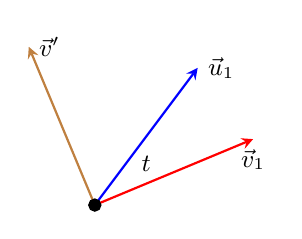
\begin{tikzpicture}
  \begin{axis}[footnotesize,font=\small
  ,axis equal,axis lines=none,samples=2, thick ]
  \addplot[black,mark=*]coordinates {(0,0)};
  \addplot[red,quiver={u=12/13,v=5/13},-stealth]coordinates {(0,0)};
  \node[below] at (axis cs:0.923,0.385) {$\vec v_1$};
  \addplot[blue,quiver={u=3/5,v=4/5},-stealth]coordinates {(0,0)};
  \node[right] at (axis cs:0.6,0.8) {$\vec u_1$};
  \addplot[brown,thick,quiver={u=-0.385,v=0.923},-stealth]coordinates {(0,0)};
  \node[right] at (axis cs:-0.385,0.923) {$\vec v'$};
  \node at (axis cs:0.3,0.24) {$t$};
  \end{axis}
\end{tikzpicture}
\end{wrapfigure}
Second, for the singular values \(\sigma_j>0\) we use a form of \idx{induction} allied with a \idx{contradiction} to prove \(\uv_j=\pm \vv_j\).
The induction starts with the case of~\(\uv_1\) and~\(\vv_1\).
We seek a \idx{contradiction} by assuming \(\uv_1\neq\pm\vv_1\)\,. Since \(\uv_1\) and~\(\vv_1\) are unit vectors, we can write \(\uv_1=\vv_1\cos t+\vv'\sin t\) for some unit vector~\(\vv'\)\ orthogonal to~\(\vv_1\) (\(\vv'\propto\Perp_{\vv_1}\uv_1\)) and for angle \(0< t<\pi\) (as illustrated above-right).
\begin{comment}
Should eliminate the possibility of \(t=\pi\)??
\end{comment}
Multiply by~\(A\) giving the identity \(A\uv_1=A\vv_1\cos t+A\vv'\sin t\)\,.
Now the first column of \(AV=US\) gives us that \(A\vv_1=\sigma_1\uv_1\)\,.
Also for the symmetric matrix \(A=\tr A=\tr{(\usv)}=V\tr S\tr U=VS\tr U\) is an alternative \svd\ of~\(A\),  
so \(AU=VS\) giving us in its first column that \(A\uv_1=\sigma_1\vv_1\)\,.
That is, the identity becomes \(\sigma_1\vv_1=\sigma_1\uv_1\cos t+(A\vv')\sin t\)\,.
Further, since \(\vv'\)~is orthogonal to~\(\vv_1\), the proof of the \svd\ \cref{thm:svd} establishes that~\(A\vv'\) is orthogonal to~\(\uv_1\).  
Equate the lengths of both sides: \(\sigma_1^2=\sigma_1^2\cos^2 t+|A\vv'|^2\sin^2 t\) which rearranging implies \((\sigma_1^2-|A\vv'|^2) \sin^2 t=0\)\,.
For angles \(0< t<\pi\) this implies \(|A\vv'|=\sigma_1\); that is, \(A\vv'=\sigma_1\uv'\) for the unit vector~\(\vv'\)\ orthogonal to~\(\vv_1\), and for some unit vector~\(\uv'\).
Hence \(\vv'\)~is a singular vector corresponding to singular value~\(\sigma_1\), and so~\(\vv'\) must also be orthogonal to \hlist[2]\vv n. Thus \(\{\vv',\hlist\vv n\}\) is an orthogonal set of unit vectors.
This is a set of \(n+1\) orthogonal vectors in \(\RR^n\) which \cref{thm:orthcomp} asserts is a contradiction.  
Hence the assumption that \(\uv_1\neq\pm\vv_1\) must be wrong.  
Consequently \(\uv_1=\pm\vv_1\) (for one of the signs, not both).

Recall the \idx{induction} proof for the \svd\ \cref{thm:svd}  (\cref{sec:dpsvdt}).  
Here, since \(\uv_1=\pm\vv_1\)\,, we can and do choose \(\bar U=\bar V\)\,.  
Hence \(B=\tr{\bar U}A\bar V =\tr{\bar V}A\bar V \) is symmetric as \(\tr{B} =\tr{(\tr{\bar V}A\bar V)} =\tr{\bar V}\tr A\bar V =\tr{\bar V}A\bar V =B\)\,.
Consequently, the same argument applies at all steps in the induction for the proof of an \svd\ and hence establishes \(\uv_j=\pm\vv_j\) (each for one of the signs, not both).

Third and last,  from the \(j\)th~column of \(AV=US\)\,, \(A\vv_j=\sigma_j\uv_j=\sigma_j(\pm \vv_j)=\lambda_j\vv_j\) for \idx{eigenvalue}~\(\lambda_j\) one of~\(\pm \sigma_j\) but not both.
\end{proof}

\begin{comment}
For duplicated \idx{singular value}s, there are \idx{eigenvector}s in the span of the \idx{singular vector}s.  
But appears difficult to prove.  
Could come down to solutions of \(Q^2=I\) for orthogonal matrix~\(Q\).
Equivalent to proving the Fundamental Theorem of Algebra that there are \(n\)~zeros of an \(n\)th~degree polynomial \pooliv{p.D8}.
\end{comment}


Recall that for every real matrix~\(A\) an \svd\ is \(A=\usv\).
But specifically for symmetric~\(A\), the proof of the previous \cref{thm:smevec} identified that the columns of~\(US\),~\(\sigma_j\uv_j\), are generally the same as~\(\lambda_j\vv_j\) and hence are the columns of~\(VD\) where \(D=\diag(\hlist\lambda n)\).
In which case the \svd\ becomes \(A=VD\tr V\).
This form of an \svd\ is intimately connected to the \text{following definition.}


\begin{definition} \label{def:odsble} 
A real \idx{square matrix}~\(A\) is \bfidx{orthogonally diagonalizable} if there exists an \idx{orthogonal matrix}~\(V\) and a \idx{diagonal matrix}~\(D\) such that \(\tr VAV=D\), equivalently \(AV=VD\), equivalently \(A=VD\tr V\) is a \idx{factorization} of~\(A\).
\end{definition}

The equivalences in this definition arise immediately from the orthogonality of matrix~\(V\) (\cref{def:orthog}): pre-multiplying \(\tr VAV=D\) by~\(V\) gives \(V\tr VAV=AV=VD\); \text{and so on.}

\needlines3
\begin{example} \label{eg:1orthdiag}
\begin{enumerate}[ref=\ref{eg:1orthdiag}(\alph*)]
\item\label[example]{eg:2x2orthdiag} Recall from \cref{eg:2x2orthevec} that the \idx{symmetric matrix} \(A=\begin{bmat} 1&3/2\\3/2&-3 \end{bmat}\) has eigenvalues \(\lambda=-\tfrac72,\tfrac32\) with corresponding orthogonal eigenvectors \((1,-3)\) and~\((3,1)\).
Normalize these eigenvectors to unit length as the columns of the orthogonal matrix
\begin{align*}
V&=\begin{bmatrix} \frac1{\sqrt{10}} & \frac3{\sqrt{10}}
\\ -\frac3{\sqrt{10}}& \frac1{\sqrt{10}} \end{bmatrix}
=\frac1{\sqrt{10}}\begin{bmatrix} 1&3\\-3&1 \end{bmatrix}
\quad\text{then}
\\\tr VAV&=\frac1{\sqrt{10}}\begin{bmatrix} 1&-3\\3&1 \end{bmatrix}
\begin{bmatrix} 1&\frac32\\\frac32&-3 \end{bmatrix}
\frac1{\sqrt{10}}\begin{bmatrix} 1&3\\-3&1 \end{bmatrix}
\\&=\frac1{10}\begin{bmatrix} -\frac72&\frac{21}2\\\frac92&\frac32 \end{bmatrix}
\begin{bmatrix} 1&3\\-3&1 \end{bmatrix}
=\frac1{10}\begin{bmatrix} -35&0\\0&15 \end{bmatrix}
=\begin{bmatrix} -\frac72&0\\0&\frac32 \end{bmatrix}.
\end{align*}
Hence this matrix is orthogonally diagonalizable.

\item Recall from \cref{eg:4x4orthevec} that the symmetric matrix
\begin{equation*}
B=\begin{bmatrix} -6 & 0 & 1 & 1
\\ 0 & 0 & 2 & 2
\\ 1 & 2 & 2 & -1
\\ 1 & 2 & -1 & -1 \end{bmatrix}
\end{equation*}
has orthogonal eigenvectors computed by \script\ into the orthogonal matrix~\verb|V|.
By additionally computing \verb|V'*B*V| we get the following diagonal result \twodp
\setbox\ajrqrbox\hbox{\qrcode{% orthogonality
B=[-6 0 1 1
 0 0 2 2
 1 2 2 -1
 1 2 -1 -1]
[V,D]=eig(B)
V'*B*V
}}%
\marginajrbox%
\begin{verbatim}
ans =
  -6.45   0.00   0.00   0.00
   0.00  -3.00   0.00  -0.00
   0.00   0.00   1.11  -0.00
  -0.00  -0.00  -0.00   3.34
\end{verbatim}
and see that this matrix~\(B\) is orthogonally diagonalizable.
\aqed
\end{enumerate}
\end{example}



These examples of orthogonal diagonalization invoke symmetric matrices.
Also, the connection between an \svd\ and orthogonal matrices was previously discussed only for symmetric matrices. 
The next theorem establishes that all real symmetric matrices are orthogonally diagonalizable, and vice versa.
That is, \idx{eigenvector}s of a matrix form an \idx{orthogonal set} if and only if the matrix is symmetric.
 

\begin{theorem}[spectral] \label{thm:symspec} 
For every real \idx{square matrix}~\(A\), 
matrix~\(A\) is symmetric iff it is \idx{orthogonally diagonalizable}.
\end{theorem}

\begin{proof} 
The ``if'' and the ``only if'' lead to two parts in the proof.
\begin{itemize}
\item If matrix~\(A\) is orthogonally diagonalizable, then \(A=VD\tr V\) for orthogonal~\(V\) and diagonal~\(D\) (and recall that for a diagonal matrix, \(\tr D=D\)).
Consider
\begin{equation*}
\tr A=\tr{(VD\tr V)}
=\tr{(\tr V)}\tr D\tr V
=VD\tr V=A\,.
\end{equation*}
Consequently the matrix~\(A\) is symmetric.

\item \cref{thm:smevec} establishes the converse for the generic case of distinct singular values.
If matrix~\(A\) is symmetric, then \cref{thm:smevec} asserts that an \svd\ \(A=\usv\) has matrix~\(U\) such that columns \(\uv_j=\pm\vv_j\)\,.
That is, we can write \(U=VR\) for diagonal matrix \(R=\diag(\pm1,\pm1,\ldots,\pm1)\) for appropriately chosen signs.
Then by the \svd\ \(A=\usv=VRS\tr V=VD\tr V\) for diagonal matrix \(D=RS=\diag(\pm\sigma_1,\pm\sigma_2,\ldots,\pm\sigma_n)\) for the same pattern of signs.
Hence matrix~\(A\) is \text{orthogonally diagonalizable.}
\end{itemize}
We omit proving the degenerate case when nonzero singular values are repeated.
\end{proof}

\begin{comment}
Further material could include the following---maybe exercises.
For every \idx{symmetric matrix}, \(A^k=VD^k\tr V\).
Also, every \idx{square matrix} has a \idx{polar decomposition} \(A=RQ\) for symmetric positive semi-definite~\(R\) and orthogonal~\(Q\) (since \(A=\usv=(US\tr U)(U\tr V)\)) \pooliv{p.610}.  
\cite{Higham86} mentions applications to the Orthogonal Procrustes problem (perhaps in approx matrices), Aerospace, Optimization, Matrix square-root, but these look too hard for this level.
\end{comment}


\index{orthogonally diagonalizable|)}
\index{diagonalizable!orthogonally|)}







\subsection{Change orthonormal basis to classify quadratics}
\label{sec:cobcqs}

\index{orthonormal basis|(}

The following preliminary example illustrates the important principle, 
applicable throughout mathematics, that we often either choose or change to a \idx{coordinate system} in which the mathematical algebra is simplest.

This optional subsection has many uses---although it is not an application itself, as it does not involve real data.


\begin{example}[choose useful coordinates] \label{eg:cuceh}
\newcommand{\myellipse}[1]{\rotatebox{30}{
\begin{tikzpicture}
  \begin{axis}[footnotesize,font=\footnotesize ,axis equal image
  , xmin=-2.5, xmax=2.5, ymin=-1.2, ymax=1.5
  , xlabel={$x$}, ylabel={$y$}
  ,axis lines=#1
  ]
  \addplot[blue,thick,smooth,domain=0:360] ({2*cos(x)},{sin(x)});
  \end{axis}
\end{tikzpicture}}}%
\newcommand{\myhyper}[1]{\rotatebox{-30}{
\begin{tikzpicture}
  \begin{axis}[footnotesize,font=\footnotesize ,axis equal image
  , xmin=-2.5, xmax=2.7, ymin=-3, ymax=3.5
  , xlabel={$x$}, ylabel={$y$}
  ,axis lines=#1
  ]
  \addplot[blue,thick,smooth,domain=-2:2] {sqrt(1+x^2*2)};
  \addplot[blue,thick,smooth,domain=-2:2] {-sqrt(1+x^2*2)};
  \end{axis}
\end{tikzpicture}}}%
Consider the following two quadratic curves. 
For each curve draw a \idx{coordinate system} in which the algebraic description of the curve would be most straightforward.

\needlines{17}
\begin{Parts}
\item Ellipse \myellipse{none}
\begin{solution} Among several possibilities is the following.\\
\myellipse{middle}\\
In this coordinate system the ellipse is algebraically \((x/2)^2+y^2=1\)\,.
\end{solution}

\item Hyperbola \myhyper{none}
\begin{solution} Possibly\\
\myhyper{middle}\\
In this coordinate system the hyperbola is algebraically \(y^2=1+2x^2\).
\end{solution}
\end{Parts}
\end{example}

Now let's proceed to see how to implement in algebra this geometric idea of choosing good coordinates to fit a given physical curve. 


\subsubsection{Graph quadratic equations}
\label{sec:gqe}
\index{quadratic equation|(}

\cref{eg:cuceh} illustrated an ellipse and a \idx{hyperbola}.  These curves are examples of the so-called \bfidx{conic section}s, which arise as solutions of the \idx{quadratic equation} in two variables, say~\(x\) and~\(y\),
\begin{equation}
ax^2+bxy+cy^2+dx+ey+f=0 \label{eq:gqe}
\end{equation}
(where \(a,b,c\) cannot all be zero).
As invoked in the example, the canonical simplest algebraic form of such curves are the following.
The challenge of this subsection is to choose good new coordinates so that a given quadratic equation~\eqref{eq:gqe} becomes one of these recognized \idx{canonical form}s.
\begin{description}
\item[Ellipse or circle] \(\frac{x^2}{a^2}+\frac{y^2}{b^2}=1\)
\begin{itemize}
\item \idx{ellipse} \(a>b\) 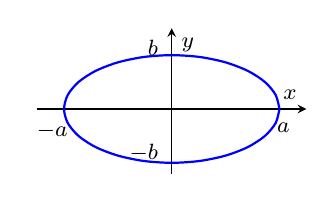
\begin{tikzpicture}
  \begin{axis}[footnotesize,font=\footnotesize ,axis equal image
  , xmin=-2.5, xmax=2.5, ymin=-1.2, ymax=1.5
  , xlabel={$x$}, ylabel={$y$}
  ,xtick={-2,2},xticklabels={$-a\quad$,$\ a$}
  ,ytick={-1,1},yticklabels={\raisebox{1.4\height}{$-b$},\raisebox{\height}{$b$}}
  ,axis lines=middle  ]
  \addplot[thick,blue,smooth,domain=0:360] ({2*cos(x)},{sin(x)});
  \end{axis}
\end{tikzpicture}

\item the \idx{circle} \(a=b\) 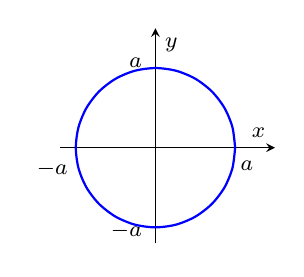
\begin{tikzpicture}
  \begin{axis}[footnotesize,font=\footnotesize ,axis equal image
  , xmin=-1.2, xmax=1.5, ymin=-1.2, ymax=1.5
  , xlabel={$x$}, ylabel={$y$}
  ,xtick={-1,1},xticklabels={$-a\qquad$,$\quad a$}
  ,ytick={-1,1},yticklabels={\raisebox{-1.6\height}{$-a$},\raisebox{1.2\height}{$a$}}
  ,axis lines=middle  ]
  \addplot[thick,blue,smooth,domain=0:360] ({cos(x)},{sin(x)});
  \end{axis}
\end{tikzpicture}

\item \idx{ellipse} \(a<b\) 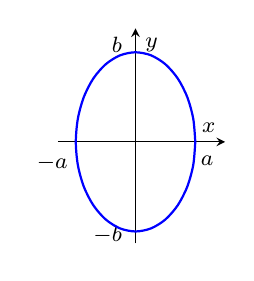
\begin{tikzpicture}
  \begin{axis}[footnotesize,font=\footnotesize ,axis equal image
  , xmin=-1.3, xmax=1.5, ymin=-1.7, ymax=1.9
  , xlabel={$x$}, ylabel={$y$}
  ,xtick={-1,1},xticklabels={$-a\qquad$,$\quad a$}
  ,ytick={-1.5,1.5},yticklabels={\raisebox{-1.4\height}{$-b$},\raisebox{\height}{$b$}}
  ,axis lines=middle  ]
  \addplot[thick,blue,smooth,domain=0:360] ({cos(x)},{1.5*sin(x)});
  \end{axis}
\end{tikzpicture}

\end{itemize}


\item[Hyperbola] \index{hyperbola}\(\frac{x^2}{a^2}-\frac{y^2}{b^2}=1\) or  \(-\frac{x^2}{a^2}+\frac{y^2}{b^2}=1\)
\begin{itemize}
\item \(\frac{x^2}{a^2}-\frac{y^2}{b^2}=1\)  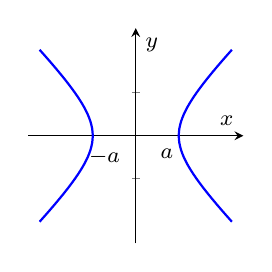
\begin{tikzpicture}
  \begin{axis}[footnotesize,font=\footnotesize ,axis equal image
  , xmin=-2.5, xmax=2.5, ymin=-2.5, ymax=2.5
  , xlabel={$x$}, ylabel={$y$}
  ,xtick={-1,1},yticklabels={{},{}}
  ,ytick={-1,1},xticklabels={$\quad-a$,$a\quad$}
  ,axis lines=middle ]
  \addplot[thick,blue,smooth,domain=-2:2] ({sqrt(1+x^2)},{x});
  \addplot[thick,blue,smooth,domain=-2:2] ({-sqrt(1+x^2)},{x});
  \end{axis}
\end{tikzpicture}

\item \(-\frac{x^2}{a^2}+\frac{y^2}{b^2}=1\)  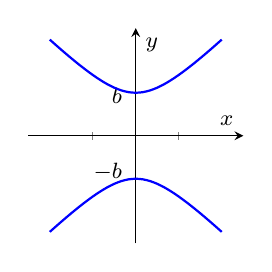
\begin{tikzpicture}
  \begin{axis}[footnotesize,font=\footnotesize ,axis equal image
  , xmin=-2.5, xmax=2.5, ymin=-2.5, ymax=2.5
  , xlabel={$x$}, ylabel={$y$}
  ,xtick={-1,1},xticklabels={{},{}}
  ,ytick={-1,1},yticklabels={\raisebox{\height}{$-b$},\raisebox{-1.4\height}{$b$}}
  ,axis lines=middle ]
  \addplot[thick,blue,smooth,domain=-2:2] {sqrt(1+x^2)};
  \addplot[thick,blue,smooth,domain=-2:2] {-sqrt(1+x^2)};
  \end{axis}
\end{tikzpicture}

\end{itemize}

\item[Parabola] \index{parabola}\(y=ax^2\) or  \(x=ay^2\)
\begin{itemize}
\item \(y=ax^2\)
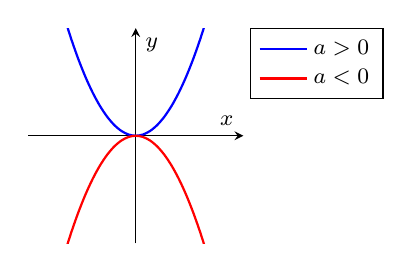
\begin{tikzpicture}
  \begin{axis}[footnotesize,font=\footnotesize ,axis equal image
  , xmin=-2.5, xmax=2.5, ymin=-2.5, ymax=2.5
  , xlabel={$x$}, ylabel={$y$}, xtick=\empty, ytick=\empty
  ,axis lines=middle, legend pos=outer north east ]
  \addplot[thick,blue,smooth,domain=-2:2] {x^2};
  \addlegendentry{$a>0$};
  \addplot[thick,red,smooth,domain=-2:2] {-x^2};
  \addlegendentry{$a<0$};
  \end{axis}
\end{tikzpicture}

\item \(x=ay^2\)
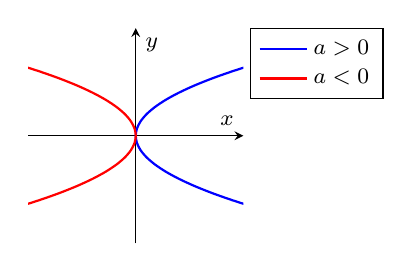
\begin{tikzpicture}
  \begin{axis}[footnotesize,font=\footnotesize ,axis equal image
  , xmin=-2.5, xmax=2.5, ymin=-2.5, ymax=2.5
  , xlabel={$x$}, ylabel={$y$}, xtick=\empty, ytick=\empty
  ,axis lines=middle, legend pos=outer north east ]
  \addplot[thick,blue,smooth,domain=-2:2] ({x^2},{x});
  \addlegendentry{$a>0$};
  \addplot[thick,red,smooth,domain=-2:2] ({-x^2},{x});
  \addlegendentry{$a<0$};
  \end{axis}
\end{tikzpicture}

\end{itemize}
\end{description}


\cref{eg:cuceh} implicitly has two steps: first, we decide upon an \idx{orientation} for the \idx{coordinate axes}; second, we decide that the \idx{coordinate system} should be `centred' in the picture.
Algebra follows the same two steps.

\begin{example}[centre coordinates] 
By shifting coordinates, identify the \idx{conic section} whose equation is
\begin{equation*}
2x^2+y^2-4x+4y+2=0\,.
\end{equation*}
\begin{solution} 
Group the linear terms with corresponding quadratic powers and seek to rewrite each as a perfect square: the equation is
\begin{eqnarray*}&&
(2x^2-4x)+(y^2+4y)+2=0
\\\iff&&
2(x^2-2x)+(y^2+4y)=-2
\\\iff&&
2(x^2-2x+1)+(y^2+4y+4)=-2+2+4
\\\iff&&
2(x-1)^2+(y+2)^2=4\,.
\end{eqnarray*}

\begin{wrapfigure}r{0pt}
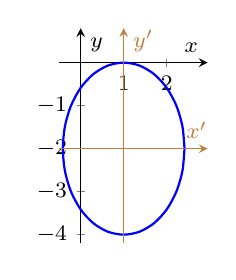
\begin{tikzpicture}
  \begin{axis}[footnotesize,font=\footnotesize ,axis equal image
  , xlabel={$x$}, ylabel={$y$}, axis lines=middle
  ]
  \addplot[blue,smooth,thick,domain=0:360] ({1+1.414*cos(x)},{-2+2*sin(x)});
  \addplot[brown,quiver={u=3.45,v=0},-stealth] coordinates {(-0.5,-2)};
  \node[brown,above] at (axis cs:2.7,-2) {$x'$};
  \addplot[brown,quiver={u=0,v=5},-stealth] coordinates {(1,-4.2)};
  \node[brown,right] at (axis cs:1,0.5) {$y'$};
  \end{axis}
\end{tikzpicture}
\end{wrapfigure}
Thus changing to a new (dashed) coordinate system \(x'=x-1\) and \(y'=y+2\)\,, that is, choosing the origin of the dashed coordinate system at \((x,y)=(1,-2)\), the quadratic equation becomes
\begin{equation*}
2{x'}^2+{y'}^2=4\,, \quad\text{that is, }
\frac{{x'}^2}{2}+\frac{{y'}^2}{4}=1\,.
\end{equation*}
In this new coordinate system the equation is that of an ellipse with horizontal axis of half-length~\(\sqrt2\) and vertical axis of half-length~\(\sqrt4=2\) (as illustrated to the right).
\end{solution}
\end{example}


\begin{example}[rotate coordinates] \label{eg:csrc2}
By rotating the \idx{coordinate system}, identify the \idx{conic section} whose equation is
\begin{equation*}
x^2+3xy-3y^2-\tfrac12=0\,.
\end{equation*}
(There are no terms linear in~\(x\) and~\(y\) so we do not shift coordinates.)
\begin{solution} 
The equation contains the product~\(xy\).
To identify the conic we must eliminate the \(xy\)~term.
To use matrix algebra, and in terms of the vector \(\xv=(x,y)\), recognize that the quadratic terms may be written as \(\tr\xv A\xv\) for symmetric matrix \(A=\begin{bmat} 1&3/2\\3/2&-3 \end{bmat}\) as then
\begin{eqnarray*}
\tr\xv A\xv
&=&\tr\xv\begin{bmatrix} 1&\frac32\\\frac32&-3 \end{bmatrix}\xv
=\begin{bmatrix} x&y \end{bmatrix}\begin{bmatrix} x+\frac32y\\\frac32x-3y \end{bmatrix}
\\&=&x(x+\tfrac32y)+y(\tfrac32x-3y)
=x^2+3xy-3y^2.
\end{eqnarray*}

\def\temp#1{\begin{tikzpicture}
  \begin{axis}[footnotesize,font=\footnotesize ,axis equal image
  , xlabel={$x$}, ylabel={$y$}, axis lines=middle
  , xtick={-1,1,2}, ytick={-2,-1,1,2}  ]
  \addplot[brown,quiver={u=1,v=-3},-stealth] coordinates {(-1/3,3/3)};
  \node[brown,right] at (axis cs:0.566,-1.7) {$x'$};
  \addplot[brown,quiver={u=0.316,v=-0.949},-stealth,thick] coordinates {(0,0)};
  \node[brown,right] at (axis cs:0.316,-0.949) {$\vec v_1$};
  \addplot[brown,quiver={u=3,v=1},-stealth] coordinates {(-3/3,-1/3)};
  \node[brown,above] at (axis cs:1.7,0.566) {$y'$};
  \addplot[brown,quiver={u=0.949,v=0.316},-stealth,thick] coordinates {(0,0)};
  \node[brown,above] at (axis cs:0.949,0.316) {$\vec v_2$};
  \ifnum#1=1
  \addplot[blue,thick,domain=-1.5:1.5] ({(x+3*sqrt(2*0.5/3+7*x^2/3))/sqrt(10)}
  ,{(-3*x+sqrt(2*0.5/3+7*x^2/3))/sqrt(10)});
  \addplot[blue,thick,domain=-1:1] ({(x-3*sqrt(2*0.5/3+7*x^2/3))/sqrt(10)}
  ,{(-3*x-sqrt(2*0.5/3+7*x^2/3))/sqrt(10)});
  \fi
  \end{axis}
\end{tikzpicture}}%
\begin{wrapfigure}r{0pt} \temp0 \end{wrapfigure}
(The matrix form \(\tr\xv A\xv\) splits the cross product term~\(3xy\) into two equal halves represented by the two off-diagonal elements~\(\tfrac32\) in matrix~\(A\).)
Suppose we change to some new (dashed) coordinate system with its \idx{standard unit vector}s~\(\vv_1\) and~\(\vv_2\) as illustrated to the right.
The vectors in the plane may then be written as the \idx{linear combination} \(\xv=\vv_1x'+\vv_2y'\).
That is, \(\xv=V\xv'\) for new coordinate vector \(\xv'=(x',y')\) and matrix \(V=\begin{bmatrix} \vv_1&\vv_2 \end{bmatrix}\).

Since the new coordinate system is related to the old by \(\xv=V\xv'\), then the quadratic terms transform as follows: 
\begin{equation*}
\tr\xv A\xv
=\tr{(V\xv')} A(V\xv')
=\tr{\xv'}\tr VAV\xv'
=\tr{\xv'}(\tr VAV)\xv'.
\end{equation*}
Thus choose~\(V\) to simplify \(\tr VAV\).
Because matrix~\(A\) is symmetric, \cref{thm:symspec} asserts that it is orthogonally diagonalizable (using eigenvectors).
Indeed, \cref{eg:2x2orthdiag} orthogonally diagonalized this particular matrix~\(A\), via its eigenvalues and eigenvectors, using the orthogonal matrix
\begin{equation*}
V=\begin{bmatrix} \vv_1&\vv_2 \end{bmatrix}
=\begin{bmatrix} \frac1{\sqrt{10}} & \frac3{\sqrt{10}}
\\ -\frac3{\sqrt{10}}& \frac1{\sqrt{10}} \end{bmatrix}.
\end{equation*}
Using this~\(V\), in the new dashed coordinate system (illustrated) the quadratic terms in the equation become
\begin{equation*}
\tr{\xv'}(\tr VAV)\xv'
=\tr{\xv'}D\xv'
=\tr{\xv'}\begin{bmatrix} -\tfrac72&0\\0&\tfrac32 \end{bmatrix}\xv'
=-\tfrac72{x'}^2+\tfrac32{y'}^2
\end{equation*}

\begin{wrapfigure}r{0pt} \temp1 \end{wrapfigure}
Hence the quadratic equation becomes
\begin{equation*}
-\tfrac72{x'}^2+\tfrac32{y'}^2-\tfrac12=0
\iff -7{x'}^2+3{y'}^2=1
\end{equation*}
which is the equation of a hyperbola intersecting the \(y'\)-axis at \(y'=\pm1/\sqrt3\)\,, as illustrated to the right.
\aqed

\end{solution}
\end{example}





\begin{example} \label{eg:cstrrc2}
Identify the \idx{conic section} whose equation is
\begin{equation*}
x^2-xy+y^2+\tfrac5{2\sqrt2}x-\tfrac7{2\sqrt2}y+\tfrac18=0\,.
\end{equation*}
\begin{solution} 
When there are both the cross product~\(xy\) and linear terms, it is  easier to first rotate coordinates, and second shift coordinates. 
\begin{enumerate}
\item Rewrite the quadratic terms using vector \(\xv=(x,y)\), splitting the cross product into two equal halves:
\begin{eqnarray*}
x^2-xy+y^2
&=&x(x-\tfrac12y)+y(-\tfrac12x+y)
=\begin{bmatrix} x&y \end{bmatrix}
\begin{bmatrix} x-\tfrac12y\\-\tfrac12x+y \end{bmatrix}
\\&=&\tr\xv 
\begin{bmatrix} 1&-\tfrac12\\-\tfrac12&1 \end{bmatrix}
\begin{bmatrix} x\\y \end{bmatrix}
=\tr\xv A\xv
\quad\text{for matrix }A=
\begin{bmat} 1&-1/2\\-1/2&1 \end{bmat}.
\end{eqnarray*}


\def\temp#1{\begin{tikzpicture}
  \begin{axis}[footnotesize,font=\footnotesize ,axis equal image
  , xlabel={$x$}, ylabel={$y$}, axis lines=middle
  , xtick={-2,-1,1,2}, ytick={-2,-1,1,2}
  ]
  \addplot[brown,quiver={u=3,v=3},-stealth] coordinates {(-1,-1)};
  \node[brown,left] at (axis cs:2,2) {$x'$};
  \addplot[brown,quiver={u=0.707,v=0.707},-stealth,thick] coordinates {(0,0)};
  \node[brown,right] at (axis cs:0.707,0.707) {$\vec v_1$};
  \addplot[brown,quiver={u=-3.2,v=3.2},-stealth] coordinates {(1,-1)};
  \node[brown,below] at (axis cs:-2,2) {$y'$};
  \addplot[brown,quiver={u=-0.707,v=0.707},-stealth,thick] coordinates {(0,0)};
  \node[brown,left] at (axis cs:-0.707,0.707) {$\vec v_2$};
  \ifnum#1>0
  \addplot[red,quiver={u=3.2,v=3.2},-stealth] coordinates {(-0.354-1.5,1.061-1.5)};
  \node[red,below] at (axis cs:1.246,2.661) {$x''$};
  \addplot[red,quiver={u=-3.2,v=3.2},-stealth] coordinates {(-0.354+1.8,1.061-1.8)};
  \node[red,right] at (axis cs:-1.554,2.261) {$y''$};
  \fi
  \ifnum#1>1
  \addplot[blue,smooth,thick,domain=0:360] 
  ({-0.354+0.707*sqrt(3)*cos(x)-0.707*sin(x)}
  ,{ 1.061+0.707*sqrt(3)*cos(x)+0.707*sin(x)});
  \fi
  \end{axis}
\end{tikzpicture}}%
\begin{figbox}{\temp0}%
Recall that \cref{eg:2evals} found that the eigenvalues of this matrix are \(\lambda=\tfrac12,\tfrac32\) with corresponding orthonormal eigenvectors \(\vv_1=(1,1)/\sqrt2\) and \(\vv_2=(-1,1)/\sqrt2\), respectively.
Let's change to a new (dashed) coordinate system~\((x',y')\) with \(\vv_1\)~and~\(\vv_2\) as its standard unit vectors (as illustrated to the right). 
Then throughout the 2D-plane every vector\slash position
\begin{equation*}
\xv=\vv_1x'+\vv_2y'=\begin{bmatrix} \vv_1&\vv_2 \end{bmatrix}\begin{bmatrix} x'\\y' \end{bmatrix}=V\xv'
\end{equation*}
for orthogonal matrix 
\begin{equation*}
V=\begin{bmatrix} \vv_1&\vv_2 \end{bmatrix}
=\frac1{\sqrt2}\begin{bmatrix} 1&-1\\1&1 \end{bmatrix}.
\end{equation*}
\end{figbox}
In the new coordinates: 
\begin{itemize}
\item the quadratic terms
\begin{eqnarray*}
x^2-xy+y^2&=&\tr\xv A\xv
\\&=&\tr{(V\xv')}A(V\xv')
\\&=&\tr{\xv'}\tr VAV\xv'
\\&=&\tr{\xv'}\begin{bmatrix} \tfrac12&0\\0&\tfrac32 \end{bmatrix}\xv'
\quad(\text{as }\tr VAV=D)
\\&=&\tfrac12{x'}^2+\tfrac32{y'}^2;
\end{eqnarray*}
\item whereas the linear terms
\begin{eqnarray*}
\tfrac5{2\sqrt2}x-\tfrac7{2\sqrt2}y
&=&\begin{bmatrix} \tfrac5{2\sqrt2}&-\tfrac7{2\sqrt2} \end{bmatrix}\xv
\\&=&\begin{bmatrix} \tfrac5{2\sqrt2}&-\tfrac7{2\sqrt2} \end{bmatrix}V\xv'
\\&=&\begin{bmatrix} -\tfrac12&-3 \end{bmatrix}\xv'
\\&=&-\tfrac12x'-3y';
\end{eqnarray*}
\item so the quadratic equation transforms to
\begin{equation*}
\tfrac12{x'}^2+\tfrac32{y'}^2-\tfrac12x'-3y'+\tfrac18=0\,.
\end{equation*}
\end{itemize}

\item 
\begin{figbox}{\temp1}%
The second step is to shift coordinates via completing the squares:
\begin{eqnarray*}
&&\tfrac12{x'}^2+\tfrac32{y'}^2-\tfrac12x'-3y'+\tfrac18=0
\\\iff&&
\tfrac12({x'}^2-x')+\tfrac32({y'}^2-2y')=-\tfrac18
\\\iff&&
\tfrac12({x'}^2-x'+\tfrac14)+\tfrac32({y'}^2-2y'+1)=-\tfrac18+\tfrac18+\tfrac32
\\\iff&&
\tfrac12(x'-\tfrac12)^2+\tfrac32(y'-1)^2=\tfrac32
\end{eqnarray*}
\end{figbox}

\begin{figbox}{\temp2}%
Thus let's change to a new (double dashed) coordinate system \(x''=x'-\tfrac12\) and \(y''=y'-1\) (equivalently, choose the origin of a new coordinate system to be at \((x',y')=(\tfrac12,1)\) as illustrated above-right).
In this new coordinate system the quadratic equation becomes
\begin{equation*}
\tfrac12{x''}^2+\tfrac32{y''}^2=\tfrac32,
\quad\text{that is } \frac{{x''}^2}3+\frac{{y''}^2}1=1\,.
\end{equation*}
In this new coordinate system the equation is that of an ellipse with \(x''\)-axis of half-length~\(\sqrt3\) and \(y''\)-axis of half-length~\(1\) (as illustrated to the right).
\aqed
\end{figbox}
\end{enumerate}
\end{solution}
\end{example}




\begin{comment}
Should include classification of 3D surfaces, but write later. 
Further motivate the following quadratic forms by mentioning some more applications.
\end{comment}

\index{quadratic equation|)}





\subsubsection{Simplify quadratic forms}
\index{quadratic form|(}


To understand the response and strength of built structures like bridges, buildings, and cars, engineers need to analyse the dynamics of energy distribution in the structure.
The potential energy in such structures is expressed and analysed as the following quadratic form.
Such quadratic forms are also important in distinguishing maxima from minima in \text{economic optimization.}

\begin{definition} \label{def:qufo}
A \bfidx{quadratic form} in variables \(\xv\in\RR^n\) is a function \(q:\RR^n\to\RR\) that may be written as \(q(\xv)=\tr\xv A\xv\) for some real symmetric \(n\times n\) matrix~\(A\).
\end{definition}

\begin{example} 
\begin{enumerate}
\item The \idx{dot product} of a vector with itself is a quadratic form.
For all \(\xv\in\RR^n\) consider
\begin{equation*}
\xv\cdot\xv=\tr\xv\xv=\tr\xv I_n\xv\,,
\end{equation*}
which is the quadratic form associated with the \idx{identity matrix}~\(I_n\).


\item \cref{eg:csrc2} found the \idx{hyperbola} satisfying equation \(x^2+3xy-3y^2-\tfrac12=0\)\,.
This equation may be written in terms of a quadratic form as \(\tr\xv A\xv-\tfrac12=0\) for vector \(\xv=(x,y)\) and \idx{symmetric matrix} \(A=\begin{bmat} 1&3/2\\3/2&-3 \end{bmat}\).


\item \cref{eg:cstrrc2} found the \idx{ellipse} satisfying the equation
\(x^2-xy+y^2+\tfrac5{2\sqrt2}x-\tfrac7{2\sqrt2}y+\tfrac18=0\) via writing the quadratic part of the equation as \(\tr\xv A\xv\) for vector \(\xv=(x,y)\) and symmetric matrix \(A=\begin{bmat} 1&-1/2\\-1/2&1 \end{bmat}\).
\end{enumerate}
\end{example}


\begin{theorem}[\idx{principal axes}] \label{thm:patqform}
For every \idx{quadratic form}, there exists an \idx{orthogonal} \idx{coordinate system} that diagonalizes the quadratic form.
Specifically, for the quadratic form~\(\tr\xv A\xv\) find the 
\idx{eigenvalue}s~\hlist\lambda n\ and an \idx{orthonormal set} of \idx{eigenvector}s~\hlist\vv n\ of symmetric~\(A\), and then in the new coordinate system~\((\hlist yn)\) with \idx{unit vector}s \(\{\hlist\vv n\}\) the quadratic form has the \bfidx{canonical form} \(\tr\xv A\xv=\lambda_1y_1^2+\lambda_2y_2^2+\cdots+\lambda_ny_n^2\).
\end{theorem}

\begin{proof} 
In the new coordinate system~\((\hlist yn)\) the orthonormal vectors~\hlist\vv n\ (called the \bfidx{principal axes}) act as the standard unit vectors.
Hence any vector \(\xv\in\RR^n\) may be written as a linear combination
\begin{equation*}
\xv=\lincomb y\vv n
=\begin{bmatrix} \vv_1&\vv_2&\cdots&\vv_n \end{bmatrix}\begin{bmatrix} y_1\\y_2\\\vdots\\y_n \end{bmatrix}
=V\yv
\end{equation*}
for orthogonal matrix \(V=\begin{bmatrix} \vv_1&\vv_2&\cdots&\vv_n \end{bmatrix}\) and vector \(\yv=(\hlist yn)\).
Then the quadratic form 
\begin{equation*}
\tr\xv A\xv=\tr{(V\yv)} A(V\yv)=\tr\yv \tr VAV\yv=\tr\yv D\yv\,,
\end{equation*}
since \(\tr VAV=D=\diag(\hlist\lambda n)\) by \cref{thm:symspec}.
Consequently,
\begin{equation*}
\tr\xv A\xv=\tr\yv D\yv=\lambda_1y_1^2+\lambda_2y_2^2+\cdots+\lambda_ny_n^2.
\end{equation*}
\end{proof}



\begin{comment}
Maybe applications to moment of inertia? and the rotating lunch box?
extreme stresses in a solid?
Could link to SVD and extreme values of length \(|A\xv|\): but where is it best established?
\end{comment}




\begin{wrapfigure}r{0pt}
\qview{28}{33}{\begin{tikzpicture} 
\begin{axis}[footnotesize,font=\footnotesize,view={\q}{60}
    ,domain=-1.3:1.3,zmin=-5
    ,xlabel={$x$},ylabel={$y$},label shift={-1.5ex}]
    \addplot3[surf,opacity=0.5] {x^2+3*x*y-3*y^2};
    \addplot3[samples y=0,domain=0:360,smooth,thick] 
    ({cos(x)},{sin(x)},{cos(x)^2+3*cos(x)*sin(x)-3*sin(x)^2});
    \addplot3[samples y=0,domain=0:360,smooth] 
    ({cos(x)},{sin(x)},{-5});
\end{axis}
\end{tikzpicture}}
\end{wrapfigure}
\begin{example} 
Consider the quadratic form \(f(x,y)=x^2+3xy-3y^2\). 
That is, consider \(f(\xv)=\tr\xv A\xv\) for \(\xv=(x,y)\) and matrix \(A=\begin{bmat} 1&3/2\\3/2&-3 \end{bmat}\).
The stereo illustration to the right shows the surface~\(f(x,y)\).
Also plotted in black is the curve of values of~\(f(x,y)\) on the unit \idx{circle} \(x^2+y^2=1\) (also shown); that is, \(f(\xv)\)~for unit vectors~\xv.
Find the maxima and minima of~\(f\) on this unit circle (for unit vectors~\xv).
Relate to the \idx{eigenvalue}s of \cref{eg:2x2orthevec}.

\begin{solution} 
Let's express the unit vectors as \(\xv=(\cos t,\sin t)\) and consider~\(f\) as a function of~\(t\).
Then 
\begin{eqnarray*}
f(t)&=&x^2+3xy-3y^2\quad(\text{for }x=\cos t\text{ and }y=\sin t)
\\&=&\cos^2t+3\cos t\sin t-3\sin^2t
\\&=&\tfrac12+\tfrac12\cos2t+\tfrac32\sin2t -\tfrac32+\tfrac32\cos2t
\\&=&-1+2\cos2t+\tfrac32\sin2t\,.
\end{eqnarray*}
From calculus, maxima and minima occur when the derivative is zero, \(df/dt=0\)\,.
Here \(df/dt=-4\sin2t+3\cos2t\) which to be zero requires \(4\sin2t=3\cos2t\)\,, that is, \(\tan2t=\tfrac34\)\,.
From the classic Pythagorean triplet of the \(3:4:5\) triangle, this tangent being~\(3/4\) requires either \begin{itemize}
\item \(\cos2t=\tfrac45\) and \(\sin2t=\tfrac35\) giving the function value \(f(t)=-1+2\cdot\tfrac45+\tfrac32\cdot\tfrac35
=\tfrac32=1.5\)\,,
\item or the negative \(\cos2t=-\tfrac45\) and \(\sin2t=-\tfrac35\) giving the function value \(f(t)=-1-2\cdot\tfrac45-\tfrac32\cdot\tfrac35
=-\tfrac72=-3.5\)\,.
\end{itemize}
These maximum and minimum values of~\(f\) seem reasonable from the plot.
Observe that these extreme values are precisely the two eigenvalues of the matrix~\(A\)---the next theorem shows this connection is no accident.
\end{solution}
\end{example}





\begin{theorem}%[Rayleigh's inequality] %?
\label{thm:optqform}
Let~\(A\) be an \(n\times n\) \idx{symmetric matrix} with \idx{eigenvalue}s \(\lambda_1\leq\lambda_2\leq\cdots\leq\lambda_n\) (sorted). 
Then for every \idx{unit vector} \(\xv\in\RR^n\) (that is, \(|\xv|=1\)), the \idx{quadratic form}~\(\tr\xv A\xv\) has the \text{following properties:}
\begin{enumerate}
\item \(\lambda_1\leq \tr\xv A\xv\leq\lambda_n\)\,;
\item the \idx{minimum} of~\(\tr\xv A\xv\) is~\(\lambda_1\), and occurs when \(\xv\) is a unit \idx{eigenvector} corresponding to~\(\lambda_1\);
\item the \idx{maximum} of~\(\tr\xv A\xv\) is~\(\lambda_n\), and occurs when \(\xv\) is a unit \idx{eigenvector} corresponding to~\(\lambda_n\).
\end{enumerate}
\end{theorem}

\begin{proof} 
Change to an orthogonal coordinate system~\yv\ that diagonalizes the matrix~\(A\) (\cref{thm:patqform}): say coordinates \(\yv=V\xv\) for orthogonal matrix~\(V\) whose columns are orthogonal eigenvectors of~\(A\) in order so that \(D=\tr VAV=\diag(\hlist\lambda n)\).
Then the quadratic form 
\begin{equation*}
\tr\xv A\xv=\tr{(V\yv)} A(V\yv)=\tr\yv \tr VAV\yv=\tr\yv D\yv\,.
\end{equation*}
Since \(V\)~is orthogonal it preserves lengths (\cref{thm:orthog:iv}) so the unit vector condition \(|\xv|=1\) is the same as \(|\yv|=1\)\,.
\begin{enumerate}
\item To prove the lower bound, consider
\begin{eqnarray*}
\tr\xv A\xv&=&\tr\yv D\yv
\\&=&\lambda_1y_1^2+\lambda_2y_2^2+\cdots+\lambda_ny_n^2
\\&=&\lambda_1y_1^2+\lambda_1y_2^2+\cdots+\lambda_1y_n^2
\\&&\quad{}
+\underbrace{(\lambda_2-\lambda_1)y_2^2}_{\geq0}
+\cdots+\underbrace{(\lambda_n-\lambda_1)y_n^2}_{\geq0}
\\&\geq&\lambda_1y_1^2+\lambda_1y_2^2+\cdots+\lambda_1y_n^2
\\&&{}=\lambda_1(y_1^2+y_2^2+\cdots+y_n^2)
=\lambda_1|\yv|^2
=\lambda_1\,.
\end{eqnarray*}
Similarly for the upper bound (\cref{ex:optqform}).  
Thus \(\lambda_1\leq \tr\xv A\xv\leq\lambda_n\) for all unit vectors~\xv.

\item Let \(\vv_1\) be a unit eigenvector of~\(A\) corresponding to the minimal eigenvalue~\(\lambda_1\); that is, \(A\vv_1=\lambda_1\vv_1\) and \(|\vv_1|=1\)\,.
Then, setting \(\xv=\vv_1\)\,, the quadratic form
\begin{equation*}
\tr\xv A\xv=\tr\vv_1A\vv_1
=\tr\vv_1\lambda_1\vv_1
=\lambda_1(\tr\vv_1\vv_1)
=\lambda_1|\vv_1|^2
=\lambda_1\,.
\end{equation*}
Thus the quadratic form~\(\tr\xv A\xv\) takes on the minimum value~\(\lambda_1\) and it occurs when \(\xv=\vv_1\) (at least).

\item \cref{ex:optqform} proves the maximum value occurs.
\end{enumerate}
\end{proof}


\begin{activity}
Recall that \cref{eg:3x3hande} found that the \(3\times3\) \idx{symmetric matrix}
\begin{equation*}
A=\begin{bmatrix} -2&0&-6\\0&4&6\\-6&6&-9 \end{bmatrix}
\end{equation*}
has \idx{eigenvalue}s \(7\), \(0\), and~\(-14\).
\begin{itemize}
\item What is the \idx{maximum} of the quadratic form \(\tr\xv A\xv\) over \idx{unit vector}s~\xv?
\actposs[4]{\(7\)}{\(-14\)}{\(0\)}{\(14\)}
\item Further, what is the \idx{minimum} of the quadratic form \(\tr\xv A\xv\) over unit vectors~\xv?
\end{itemize}
\end{activity}

\index{orthonormal basis|)}


\begin{comment}
Could define positive/negative semi-definite forms/matrices.
But seems incidental so do not write yet.
\end{comment}




\begin{comment}  
Could have an optional application section on the following problem: useful whenever we can assess any pair of items, but do not have a framework for their absolute position.
Find \(m\) points in \(n\)D given that you know their distance
matrix and given that the mean location is precisely zero
\cite[p.83]{Hopcroft2014}. 
See \verb|multiDscaling.m|
\end{comment}


\index{quadratic form|)}





\sectionExercises


\begin{exercise}  
Each plot below shows (unit) vectors~\xv\ (blue), and for some \(2\times 2\) matrix~\(A\) the corresponding vectors~\(A\xv\) (red) adjoined. 
By assessing whether there are any zero eigenvalues, estimate if the matrix~\(A\) is \idx{invertible} \text{or not.}

\begin{Parts}
%\def\eRosesize{small}
\item\eRose{1}{-0.8}{-0.8}{1.5}%sym
\answer{invertible}

\item\eRose{0.5}{0.4}{1}{0.8}
\answer{not invertible}

\begin{OmitV1}
\item\eRose{-0.5}{0.2}{1.3}{0.4}
\answer{invertible}

\item\eRose{0.2}{-0.5}{-0.4}{1.0}%sym
\answer{not invertible}
\end{OmitV1}

\item\eRose{1.0}{-0.25}{-1.2}{0.3}
\answer{not invertible}

\item\eRose{-0.2}{0.2}{-0.3}{-0.45}
\answer{invertible}

\end{Parts}
\end{exercise}


\begin{exercise}  
For each of the following symmetric matrices, from a hand derivation of the \idx{characteristic equation} (defined in \cref{pro:eeh}), determine whether each matrix has a zero \idx{eigenvalue} or not, and hence determine whether it is \idx{invertible} \text{or not.}
\begin{Parts}
\item \(\begin{bmatrix} -1/2 & -3/4
\\ -3/4 & -1/2 \end{bmatrix}\)
\answer{eigenvalues \(-5/4,1/4\) so invertible.}

\item \(\begin{bmatrix} 4 & -2
\\ -2 & 1 \end{bmatrix}\)
\answer{eigenvalues \(0,5\) so not invertible.}

\item \(\begin{bmatrix} 0 & -2/5
\\ -2/5 & 3/5 \end{bmatrix}\)
\answer{eigenvalues \(-1/5,4/5\) so invertible.}

\item \(\begin{bmatrix} 2 & 1 & -2
\\ 1 & 3 & -1
\\ -2 & -1 & 2 \end{bmatrix}\)
\answer{eigenvalues \( 0,2,5\) so not invertible.}

\begin{OmitV1}
\item \(\begin{bmatrix} -2 & -1 & 1
\\ -1 & -0 & -1
\\ 1 & -1 & -2 \end{bmatrix}\)
\answer{eigenvalues \(-3,-2,1\) so invertible.}

\item \(\begin{bmatrix} 2 & 1 & 1
\\ 1 & 2 & 1
\\ 1 & 1 & 2 \end{bmatrix}\)
\answer{eigenvalues \(1,4\) so invertible.}

\item \(\begin{bmatrix} -1/2 & 3/2 & 1
\\ 3/2 & -3 & -3/2
\\ 1 & -3/2 & -1/2 \end{bmatrix}\)
\answer{eigenvalues \(-9/2,0,1/2\) so not invertible.}

\item \(\begin{bmatrix} 1 & -1 & -1
\\ -1 & -1/2 & 1/2
\\ -1 & 1/2 & -1/2 \end{bmatrix}\)
\answer{eigenvalues \(-1,2\) so invertible.}
\end{OmitV1}


\end{Parts}
%\begin{comment}
%obtain via brutal search
%\begin{verbatim}
%format rat
%n=3
%for i=1:10^(n-1)
%k=ceil(5*rand);
%a=eye(n)/2+randn(n); a=round((a+a')*k)/k;
%d=eig(a)'; [dn,dd]=rat(d,1e-7);
%if max(abs(dd))<10, AD=[a;d], end
%end
%\end{verbatim}
%\end{comment}
\end{exercise}





\begin{exercise} \label{ex:smoevs} 
For each of the following (symmetric) matrices, find by hand the \idx{eigenvalue}s and \idx{eigenvector}s.  
Using these eigenvectors, confirm that the eigenvalues of the matrix squared are the square of its eigenvalues.
If the matrix has an \idx{inverse}, what are the eigenvalues of \text{the inverse?}

%\begin{verbatim}
%format rat,n=3
%for i=1:10^n
%k=ceil(2*rand); a=eye(n)/2+randn(n); a=0+round((a+a')*k)/k;
%[v,d]=eig(a); [dn,dd]=rat(diag(d),1e-7);
%if max(abs(dd))<10, A=a, d=diag(d)', vd=diag(1./max(abs(v)))*(v'), break, end
%end
%\end{verbatim}
\begin{Parts}
\item \(\eAii=\begin{bmatrix} 0&-2
\\-2&3 \end{bmatrix}\)
\answer{Eigenvalues \(-1,4\), and corresponding eigenvectors proportional to \((2,1)\), \((-1,2)\).
The inverse has eigenvalues \(-1,1/4\).}

\item \(\eAii=\begin{bmatrix} 5/2&-2
\\-2&5/2 \end{bmatrix}\)
\answer{Eigenvalues \(1/2,9/2\), and corresponding eigenvectors proportional to \((1,1)\), \((-1,1)\).
The inverse has eigenvalues \(2,2/9\).}

\begin{OmitV1}
\item \(\eAii=\begin{bmatrix} 3&8
\\8&-9 \end{bmatrix}\)
\answer{Eigenvalues \(-13,7\), and corresponding eigenvectors proportional to \((-1,2)\), \((2,1)\).
The inverse has eigenvalues \(-1/13,1/7\).}

\item \(\eAii=\begin{bmatrix} -2&1
\\1&14/5 \end{bmatrix}\)
\answer{Eigenvalues \(-11/5,3\), and corresponding eigenvectors proportional to \((-5,1)\), \((1,5)\).
The inverse has eigenvalues \(-5/11,1/3\).}

\item \(\eAii=\begin{bmatrix} -1&-2&0
\\-2&0&2
\\0&2&1 \end{bmatrix}\)
\answer{Eigenvalues \(-3,0,3\), and corresponding eigenvectors proportional to \((2,2,-1)\), \((2,-1,2)\), \((-1,2,2)\).
The inverse does not exist.}

\item \(\eAii=\begin{bmatrix} 2&1&3
\\1&0&-1
\\3&-1&2 \end{bmatrix}\)
\answer{Eigenvalues \(-2,1,5\), and corresponding eigenvectors proportional to \((-1,1,1)\), \((1,2,-1)\), \((1,0,1)\).
The inverse has eigenvalues \(-1/2,1,1/5\).}
\end{OmitV1}

\item \(\eAii=\begin{bmatrix} 0&-1&-1
\\-1&1&0
\\-1&0&1 \end{bmatrix}\)
\answer{Eigenvalues \(-1,1,2\), and corresponding eigenvectors proportional to \((2,1,1)\), \((0,-1,1)\), \((1,-1,-1)\).
The inverse has eigenvalues \(-1,1,1/2\).}

\item \(\eAii=\begin{bmatrix} -1&3/2&3/2
\\3/2&-3&-1/2
\\3/2&-1/2&3 \end{bmatrix}\)
\answer{Eigenvalues \(-4,-1/2,7/2\), and corresponding eigenvectors proportional to \((-3,5,1)\), \((3,2,-1)\), \((1,0,3)\).
The inverse has eigenvalues \(-1/4,-2,2/7\).}

\end{Parts}
\end{exercise}





\begin{exercise}  
Each plot below shows (unit) vectors~\xv\ (blue), and for some \(2\times 2\) matrix~\(A\) the corresponding vectors~\(A\xv\) (red) adjoined. 
For each plot of a matrix~\(A\) there is a companion plot for the \idx{inverse matrix}~\(A^{-1}\).
By roughly estimating \idx{eigenvalue}s and \idx{eigenvector}s by eye, identify the pairs of plots corresponding to each matrix and \text{its inverse.}
\begin{Parts}
\item\label{ex:epria} \eRose{1.9}{-1.9}{-1.9}{3.3}
\item\label{ex:eprib} \eRose{2.7}{1.2}{1.2}{-2.}
\item\label{ex:epric} \eRose{0.3}{0.7}{0.7}{0.1}
\item\label{ex:eprid} \eRose{0.2924}{0.17544}{0.17544}{-0.39474}
\begin{OmitV1}
\item\label{ex:eprie} \eRose{0.93333}{0.2}{0.2}{0.4}
\item\label{ex:eprif} \eRose{1.2}{-0.6}{-0.6}{2.8}
\item\label{ex:eprig} \eRose{0.836364}{-0.036364}{-0.036364}{0.436364}
\end{OmitV1}
\item\label{ex:eprih} \eRose{1.2406}{0.71429}{0.71429}{0.71429}
\item\label{ex:eprii} \eRose{-0.21739}{1.52174}{1.52174}{-0.65217}
\begin{OmitV1}
\item\label{ex:eprij} \eRose{1.2}{0.1}{0.1}{2.3}
\end{OmitV1}
\end{Parts}
\answer{Some pairs are \ref{ex:epria}-\ref{ex:eprih}
,\ref{ex:eprid}-\ref{ex:eprid}
,\ref{ex:epric}-\ref{ex:eprii}
%,\ref{ex:eprie}-\ref{ex:eprif}
%,\ref{ex:eprig}-\ref{ex:eprij}
}
%\begin{comment} try some, choose, then random order
%\begin{verbatim}
%for i=1:9
%a=eye(2)/2+randn(2)/2; a=round((a+a')*10)/10;
%b=inv(a);
%Ainv=[a(:)';b(:)']
%end
%\end{verbatim}
%\end{comment}
\end{exercise}





\begin{exercise}  
For the symmetric matrices of \cref{ex:smoevs}, confirm that \idx{eigenvector}s corresponding to \idx{distinct eigenvalues} are orthogonal (\cref{thm:orthoevec}).  
Show your working.
\end{exercise}






\begin{exercise}  
For every \(n\times n\) \idx{symmetric matrix},
\begin{itemize}
\item  eigenvectors corresponding to distinct eigenvalues are orthogonal (\cref{thm:orthoevec}), and
\item  there are generally \(n\)~eigenvalues.
\end{itemize}
Which of the illustrated 2D examples of \cref{ex:evecpic} appear to come from symmetric matrices, and which appear to come from non-symmetric matrices?
\end{exercise}





\begin{exercise} \label{ex:smnoevs} 
For each of the following \emph{non-symmetric} matrices, confirm that \idx{eigenvector}s corresponding to \idx{distinct eigenvalues} are \emph{not} orthogonal.  Show and comment on your working.
Find eigenvectors by hand for \(2\times 2\) and \(3\times 3\) matrices, and compute with \script\ for \(4\times 4\) matrices and larger (using \verb|eig()| and \verb|V'*V|).
%\begin{verbatim}
%format rat,n=2
%for i=1:10^n
%a=0+round(randn(n)*4); 
%[v,d]=eig(a); [dn,dd]=rat(diag(d),1e-7);
%if max(abs(dd))<10, A=a, d=diag(d)', vd=diag(1./max(abs(v)))*(v'), break, end
%end
%\end{verbatim}
\begin{Parts}
\item \(\eAii=\begin{bmatrix} -2&2
\\3&-3 \end{bmatrix}\)
\answer{Eigenvectors proportional to \((1,1)\), \((-2,3)\).}

\begin{OmitV1}
\item \(\eAii=\begin{bmatrix}1&-3
\\-2&2 \end{bmatrix}\)
\answer{Eigenvectors proportional to \((3,2)\), \((1,-1)\).}

\item \(\eAii=\begin{bmatrix} 1&-2&6
\\4&3&2
\\-3&1&-8 \end{bmatrix}\)
\answer{Eigenvectors proportional to \((-2,3,1)\), \((2,-2,-1)\), \((-13,3,14)\).}
\end{OmitV1}

\item \(\eAii=\begin{bmatrix} -1&-2&9
\\3&-6&3
\\0&0&3 \end{bmatrix}\)
\answer{Eigenvectors proportional to \((1,1,0)\), \((2,3,0)\), \((25,13,14)\).}

%\begin{verbatim}
%format short, n=5; A=eye(n)+round(randn(n)*3), [v,d]=eig(A); d=diag(d)', format bank, vd=v'
%\end{verbatim}

\item \(\eAii=\begin{bmatrix} 2&1&-2&1
\\1&-3&4&-4
\\3&2&4&-5
\\-3&-1&-3&0 \end{bmatrix}\)
\answer{Eigenvectors proportional to \((-.39,.44,.76,-.28)\), \((.58,-.41,-.68,.18)\), \((.22,-.94,.23,.11)\), \((.21,-.53,.53,.62)\) \twodp.}

\begin{OmitV1}
\item \(\eAii=\begin{bmatrix} -4&0&-5&7
\\2&3&1&-3
\\1&4&-2&4
\\1&-3&4&2 \end{bmatrix}\)
\answer{Eigenvectors proportional to \((-.89,.27,-.24,.28)\), \((-.86,.28,.43,-.01)\), \((-.38,.68,.62,.09)\), \((.44,-.45,.21,.75)\) \twodp.}

\item \(\eAii=\begin{bmatrix} 1&4&3&1&-1
\\5&1&6&-0&1
\\0&4&-3&1&4
\\-3&2&1&4&-1
\\-2&2&2&2&1 \end{bmatrix}\)
\answer{Eigenvectors proportional to \((.01,-.63,.78,.04,-.05)\), \((-.59,.49,.21,-.46,-.39)\), \((.57,.74,.33,-.01,.15)\), \((-.46,-.46,.07,.62,.43)\), \((-.52,-.07,.32,-.53,.59)\) \twodp.}
\end{OmitV1}

\item \(\eAii=\begin{bmatrix} 2&0&2&-1&-1
\\2&1&-1&2&-0
\\5&-2&6&2&-1
\\4&0&-2&6&-5
\\2&0&-5&-3&-5 \end{bmatrix}\)
\answer{Eigenvectors proportional to \((.20,-.19,-.10,.32,.90)\), \((.40,-.53,-.35,.12,.65)\), \((-.47,-.83,.03,.18,-.24)\), \((-.24,-.06,-.82,-.39,.35)\), \((.28,-.27,.26,-.87,.17)\) \twodp.}

\end{Parts}
\end{exercise}




\begin{exercise}  
For the symmetric matrices of \cref{ex:smoevs}, use \script\ to compute an \svd\ (\(\usv\)) of each matrix.
Confirm that each column of~\(V\) is an \idx{eigenvector} of the matrix (that is, proportional to what the exercise found) and the corresponding \idx{singular value} is the \idx{magnitude} of the corresponding \idx{eigenvalue} (\cref{thm:smevec}).
Show and discuss \text{your working.}
\end{exercise}




\begin{exercise}  
To complement the previous exercise, for each of the \emph{non-symmetric} matrices of \cref{ex:smnoevs}, use \script\ to compute an \svd\ (\(\usv\)) of each matrix.
Confirm that usually each column of~\(V\) is \emph{not} an \idx{eigenvector} of the matrix, and the \idx{singular value}s do \emph{not} appear closely related to the \idx{eigenvalue}s.
Show and discuss \text{your working.}
\end{exercise}











\begin{exercise}  
Let \(A\) be an \(m\times n\)  matrix with \svd\ \(A=\usv\).
Prove that for any \(j=1,2,\ldots,n\)\,, the \(j\)th~column of~\(V\),~\(\vv_j\), is an \idx{eigenvector} of the \(n\times n\) {symmetric matrix}~\(\tr AA\) corresponding to the \idx{eigenvalue} \(\lambda_j=\sigma_j^2\) (or \(\lambda_j=0\) if \(m<j\leq n\)).
%Further, if \(A\)~is  an \(n\times n\) \idx{symmetric matrix}, then \(\vv_j\)~is an eigenvector of~\(A^2\) corresponding to the eigenvalue~\(\sigma_j^2\).
\end{exercise}



\begin{exercise} \label{ex:ematpow:iii} 
Prove \cref{thm:ematpow:iii} using parts~\ref{thm:ematpow:i} 
and~\ref{thm:ematpow:ii}: that if matrix~\(A\) is {invertible}, then 
for every integer~\(n\) (including negative~\(n\)), \(\lambda^n\) is an \idx{eigenvalue} 
of~\(A^n\) with corresponding \idx{eigenvector}~\xv.
\end{exercise}





\begin{exercise}  
For each of the following matrices, give reasons as to whether the matrix is \idx{orthogonally diagonalizable}, and if it is, then find an \idx{orthogonal matrix}~\(V\) that does so and the corresponding \idx{diagonal matrix}~\(D\).
Use \script\ for the larger matrices.
%\begin{verbatim}
%format rat,n=4
%for i=1:10^n
%k=ceil(3*rand); a=eye(n)/2+randn(n); a=0+round((a+(rand<1)*a')*k)/k;
%[v,d]=eig(a); [dn,dd]=rat(diag(d),1e-7);
%if max(abs(dd))<10, A=a, d=diag(d)', vv=v*diag(1./max(abs(v))), break, end
%end
%\end{verbatim}

\begin{Parts}
\begin{OmitV1}
\item \(\eAii=\begin{bmatrix} 0&-2/3
\\-1&-1/3 \end{bmatrix}\)
\answer{Not symmetric, so not orthogonally diagonalizable.}

\item \(\eAii=\begin{bmatrix} 2/3&2
\\2&7/3 \end{bmatrix}\)
\answer{\(V=\frac1{\sqrt{13}}\protect\begin{bmat} -3&2
\protect\\2&3 \protect\end{bmat}\), 
and \(D=\diag(-2/3,11/3)\).}
\end{OmitV1}

\item \(\eAii=\begin{bmatrix} 2&0&1
\\0&2&-1
\\1&-1&3 \end{bmatrix}\)
\answer{\(V=\protect\begin{bmat} -\fs3&\fs2&\fs6
\protect\\\fs3&\fs2&-\fs6
\protect\\\fs3&0&\fs[2]6 \protect\end{bmat}\), 
and \(D=\diag(1,2,4)\).}

\item \(\eAii=\begin{bmatrix} 2&0&2
\\1&-1&0
\\-1&0&-1 \end{bmatrix}\)
\answer{Not symmetric, so not orthogonally diagonalizable.}

\begin{OmitV1}
\item \(\eAii=\begin{bmatrix} 0&-2&-2&0
\\-2&0&-2&0
\\-2&-2&2&2
\\0&0&2&-2 \end{bmatrix}\)
\answer{\(V=\protect\begin{bmat} -.50&-.41&.71&-.29
\protect\\-.50&-.41&-.71&-.29
\protect\\-.50&.00&.00&.87
\protect\\.50&-.82&.00&.29 \protect\end{bmat}\) \twodp, 
and \(D=\diag(-4,-2,2,4)\).}

\item \(\eAii=\begin{bmatrix} -1&0&0&0
\\0&3&-2&-2
\\0&-2&0&1
\\0&-2&1&0 \end{bmatrix}\)
\answer{\(V=\protect\begin{bmat} .00&1.00&.00&.00
\protect\\.06&.00&.57&-.82
\protect\\-.64&.00&.65&.41
\protect\\.76&.00&.50&.41 \protect\end{bmat}\) \twodp, 
and \(D=\diag(-1,-1,-1,5)\).}
\end{OmitV1}

\item \(\eAii=\begin{bmatrix} 3&1&1&1&-1
\\-1&0&0&0&1
\\0&0&0&0&1
\\0&1&-1&1&-1
\\0&0&0&0&1 \end{bmatrix}\)
\answer{Not symmetric, so not orthogonally diagonalizable.}

\item \(\eAii=\begin{bmatrix} 3&0&2&0&0
\\0&3&1&0&-1
\\2&1&1&0&-1
\\0&0&0&3&2
\\0&-1&-1&2&1 \end{bmatrix}\)
\answer{\(V=\protect\begin{bmat} -.32&.37&.41&-.63&.45
\protect\\-.00&.37&-.82&-.00&.45
\protect\\.63&-.55&-.00&-.32&.45
\protect\\-.32&-.37&-.41&-.63&-.45
\protect\\.63&.55&.00&-.32&-.45 \protect\end{bmat}\) \twodp, 
and \(D=\diag(-1,0,3,4,5)\).}

\end{Parts}
\end{exercise}





\begin{exercise}  
Let matrix~\(A\) be invertible and \idx{orthogonally diagonalizable}.  
Show that the \idx{inverse}~\(A^{-1}\) is \idx{orthogonally diagonalizable}.
\end{exercise}




\begin{exercise}  
Suppose matrices~\(A\) and~\(B\) are \idx{orthogonally diagonalizable} by the same \idx{orthogonal matrix}~\(V\).  
Show that \(AB=BA\) and that the product~\(AB\) is \idx{orthogonally diagonalizable}.
\end{exercise}




\begin{exercise}  
For each of the given symmetric matrices, say~\(A\), find a symmetric matrix~\(X\) such that \(X^2=A\)\,.  
That is, find a \idx{square-root} of the matrix.
%\begin{verbatim}
%format rat,n=2
%for i=1:10^n
%k=ceil(3*rand); a=eye(n)/2+randn(n); a=0+round((a+a')*k)/k;
%[v,d]=eig(a); [dn,dd]=rat(diag(d),1e-7);
%if max(abs(dd))<10, A=a^2, X=a, d=diag(d)', vv=v*diag(1./max(abs(v))), break, end
%end
%\end{verbatim}
\begin{Parts}
\item \(\eAii=\begin{bmatrix} 5/2&3/2
\\3/2&5/2 \end{bmatrix}\)
\answer{\(X=\protect\begin{bmat} 3/2&1/2
\protect\\1/2&3/2 \protect\end{bmat}\)}

\item \(\eAii=\begin{bmatrix} 6&-5&-5
\\-5&10&1
\\-5&1&10 \end{bmatrix}\)
\answer{\(X=\protect\begin{bmat} 2&-1&-1
\protect\\-1&3&0
\protect\\-1&0&3 \protect\end{bmat}\)}

\item \(\eAii=\begin{bmatrix} 2&1&3
\\1&2&3
\\3&3&6 \end{bmatrix}\)
\answer{\(X=\protect\begin{bmat} 1&0&1
\protect\\0&1&1
\protect\\1&1&2 \protect\end{bmat}\)}

\item How many possible answers are there for each of the given matrices?  Why?
\answer{four, eight, and four respectively.}

\item For each symmetric matrix, say~\(A\), show that if every eigenvalue of~\(A\) is non-negative, then there exists a symmetric matrix~\(X\) such that \(A=X^2\).  

\item Continuing the previous part, how many such matrices~\(X\) exist?  Justify your answer.

\end{Parts}
\end{exercise}






\begin{exercise}  
For each of the following \idx{conic section}s, draw a pair of \idx{coordinate axes} for a \idx{coordinate system} in which the algebraic description of the curves should be simplest.
\newcommand{\myellipse}[3]{\rotatebox{#3}{
\begin{tikzpicture}
  \begin{axis}[footnotesize,font=\footnotesize ,axis equal image
  ,axis lines=none ]
  \addplot[blue,thick,smooth,domain=0:360] ({#1*cos(x)},{#2*sin(x)});
  \end{axis}
\end{tikzpicture}}}%
\newcommand{\myhyper}[3]{\rotatebox{#3}{
\begin{tikzpicture}
  \begin{axis}[footnotesize,font=\footnotesize ,axis equal image
  ,axis lines=none ]
  \addplot[blue,thick,smooth,domain=-2:2] {#1*sqrt(1+x^2*#2)};
  \addplot[blue,thick,smooth,domain=-2:2] {-#1*sqrt(1+x^2*#2)};
  \end{axis}
\end{tikzpicture}}}%

\begin{Parts}
\item \myellipse{1}{3}{60}
\item \myhyper{1}{3}{20}
\item \myellipse{3.01}{1.37}{10}
\item \myhyper{1.70}{1.96}{76}
\begin{OmitV1}
\item \myellipse{2.42}{3.72}{58}
\item \myhyper{2.63}{2.31}{150}
\end{OmitV1}
\end{Parts}
\end{exercise}





\begin{exercise}  
By shifting to new \idx{coordinate axes}, find the \idx{canonical form} of each of the following \idx{quadratic equation}s, and hence describe each curve. 
%\begin{verbatim}
%cs=round(randn(1,5)*4), md=-cs(3:4)./cs(1:2)/2, absq=(-cs(5)+md.^2*cs(1:2)')./cs(1:2)
%\end{verbatim}
\begin{Parts}
\item \(-4x^2+5y^2+4x+4y-1=0\)
\answer{hyperbola, centred \((1/2,-2/5)\), \(-\frac{{x'}^2}{1/5}+\frac{{y'}^2}{4/25}=1\)}

\item \(-4y^2-6x -4y +2=0\)
\answer{parabola, base \((1/2,-1/2)\), \({x'}=-\frac23{{y'}^2}\)}

\item \(5x^2-y^2 -2y +4=0\)
\answer{hyperbola, centred \((0,-1)\), \(-\frac{{x'}^2}{1}+\frac{{y'}^2}{5}=1\)}

\item \(3x^2 +5y^2 +6x +4y +2=0\)
\answer{ellipse, centred \((-1,-2/5)\), \( \frac{{x'}^2}{3/5}+\frac{{y'}^2}{9/25}=1\)}

\item \(-2x^2 -4y^2 +7x -2y +1=0\)
\answer{ellipse, centred \((7/4,-1/4)\), \( \frac{{x'}^2}{59/16}+\frac{{y'}^2}{59/32}=1\)}

\begin{OmitV1}
\item \(-9x^2-y^2 -3y +6=0\)
\answer{ellipse, centred \((0,-3/2)\), \( \frac{{x'}^2}{11/12}+\frac{{y'}^2}{33/4}=1\)}

\item \(-x^2-4x -8y +4=0\)
\answer{parabola, base \((-2,1)\), \({y'}=-\frac18{{x'}^2}\)}

\item \(-8x^2-y^2-2x +2y -3=0\)
\answer{No solution points exist.}
\end{OmitV1}

\end{Parts}
\end{exercise}






\begin{exercise}  
By rotating to new \idx{coordinate axes}, identify each of the following \idx{conic section}s.  
Write the quadratic terms in the form \(\tr\xv A\xv\), and use the eigenvalues and eigenvectors of matrix~\(A\).
%\begin{verbatim}
%for i=1:99,c=0+round(randn(1,4)*4),A=[c(1) c(2)/2;c(2)/2 c(3)],[V,D]=eig(A);VV=sign(V).*V.^2,d=diag(D)',absq=-c(4)./d,[vn,vd]=rat(VV,1e-7);if max(vd(:))<11,break,end,end
%\end{verbatim}

\begin{Parts}
\item \(4xy +3y^2 -3=0\)
\answer{With axes \(\iv'=(-\fs[2]5,\fs5)\) and \(\jv'=(\fs5,\fs[2]5)\), 
\( -\frac{{x'}^2}{3}+\frac{{y'}^2}{3/4}=1\) is hyperbola.}

\item \(3x^2 +8xy -3y^2 =0\)
\answer{With axes \(\iv'=(\fs5,-\fs[2]5)\) and \(\jv'=(\fs[2]5,\fs5)\), 
\( -5{{x'}^2}{}+5{{y'}^2}{}=0\) is pair of straight lines.}

\item \(2x^2 -3xy +6y^2 -5=0\)
\answer{In axes \(\iv'=(\fs[3]{10},\fs{10})\) and \(\jv'=(-\fs{10},\fs[3]{10})\), 
\( \frac{{x'}^2}{10/3}+\frac{{y'}^2}{10/13}=1\) is ellipse.}

\item \(-4x^2 +3xy -4y^2 -2=0\)
\answer{No solution points exist.}

\begin{OmitV1}
\item \(-4x^2 +3xy -4y^2 +11=0\)
\answer{In axes \(\iv'=(\fs2,-\fs2)\) and \(\jv'=(\fs2,\fs2)\), 
\( \frac{{x'}^2}{2}+\frac{{y'}^2}{22/5}=1\) is ellipse.}

\item \(3x^2 -2xy +3y^2 -6=0\)
\answer{In axes \(\iv'=(\fs2,\fs2)\) and \(\jv'=(-\fs2,\fs2)\), 
\( \frac{{x'}^2}{3}+\frac{{y'}^2}{3/2}=1\) is ellipse.}

\item \(-x^2 +2xy -y^2 +5=0\)
\answer{In axes \(\iv'=(\fs2,-\fs2)\) and \(\jv'=(\fs2,\fs2)\), 
\( \frac{{x'}^2}{5/2}=1\) is pair of parallel lines.}

\item \(-x^2 -4xy +2y^2 -6=0\)
\answer{In axes \(\iv'=(\fs[2]5,\fs5)\) and \(\jv'=(-\fs5,\fs[2]5)\), 
\( -\frac{{x'}^2}{3}+\frac{{y'}^2}{2}=1\) is hyperbola.}
\end{OmitV1}

\end{Parts}
\end{exercise}





\begin{exercise}  
By rotating and shifting to new \idx{coordinate axes}, identify each of the following \idx{conic section}s from its equation.
%\begin{verbatim}
%for i=1:99,c=0+round(randn(1,4)*4),A=[c(1) c(2)/2;c(2)/2 c(3)],[V,D]=eig(A);VV=sign(V).*V.^2,d=diag(D)',absq=-c(4)./d,[vn,vd]=rat(VV,1e-7);if max(vd(:))<11,break,end,end
%a=round(randn(2,1)*6)/2, angle=num2str(atan(V(2)/V(1))*180/pi)
%cs=[c(1:3) -[2 1].*c(1:2)*a -[1 2].*c(2:3)*a c(4)+a'*A*a]
%[X,Y]=meshgrid(linspace(-1,1,41)*7);
%f=cs(1)*X.^2+cs(2)*X.*Y+cs(3)*Y.^2+cs(4)*X+cs(5)*Y+cs(6);
%contour(X,Y,f,[-10 -1 -0.1 0 0.1 1 10]), axis equal
%\end{verbatim}
\begin{enumerate}
\item \( -2x^2 -5xy -2y^2 -\frac{33}2x -15y -32=0\)
\answer{hyperbola centred \((-1,-5/2)\) at angle~\(45^\circ\)}

\item \( -7x^2 +3xy -3y^2 -52x +\frac{33}2y -\frac{381}4=0\)
\answer{ellipse centred \((-7/2,1)\) at angle~\(78^\circ\)}

\item \( -4xy -3y^2 -18x -11y +\frac{37}4=0\)
\answer{hyperbola centred \((4,-9/2)\) at angle~\(-27^\circ\)}

\begin{OmitV1}
\item \( 2x^2 -y^2 +10x +6y +\frac{11}2=0\)
\answer{hyperbola centred \((-5/2,3)\) at angle~\(0^\circ\)}

\item \( -2x^2 +5xy -2y^2 -\frac{13}2x +\frac52y +\frac{31}4=0\)
\answer{hyperbola centred \((3/2,5/2)\) at angle~\(45^\circ\)}

\item \(-4xy +3y^2 +18x -13y +\frac34=0\)
\answer{hyperbola centred \((7/2,9/2)\) at angle~\(26^\circ\)}
\end{OmitV1}

\item \( 6x^2 +6y^2 -12x -42y +\frac{155}2=0\)
\answer{circle centred \((1,7/2)\)}

\item \( 2x^2 -4xy +5y^2 +34x -52y +\frac{335}2=0\)
\answer{ellipse centred \((-11/2,3)\) at angle~\(26^\circ\)}


\end{enumerate}
\end{exercise}






\begin{exercise}  
For each of the following matrices, say~\(A\), consider the corresponding \idx{quadratic form} \(q(\xv)=\tr\xv A\xv\).
Find \idx{coordinate axes}, the \idx{principal axes}, such that the quadratic has the \idx{canonical form} in the new coordinates \hlist yn.
Use eigenvalues and eigenvectors, and use \script\ for the larger matrices.
Over all unit vectors, what is the \idx{maximum} value of~\(q(\xv)\)? and what is the \idx{minimum} value?

%\begin{verbatim}
%n=2
%for i=1:999
%a=randn(n); A=0+round((a+a')*3); [V,D]=eig(A);
%VV=V.*abs(V); [vvn,vvd]=rat(VV,1e-7);
%if max(vvd(:))<13,A=A,num2str(diag(D)',"%7.2f"), VV=VV, break, end
%end
%\end{verbatim}
\begin{Parts}
\item \(\eAii=\begin{bmatrix} 0&-5
\\-5&0 \end{bmatrix}\)
\answer{\(q= -5y_1^2 +5y_2^2\), max\(=5\), min=\(-5\)}

\begin{OmitV1}
\item \(\eAii=\begin{bmatrix} 3&2
\\2&0 \end{bmatrix}\)
\answer{\(q= -y_1^2 +4y_2^2\), max\(=4\), min=\(-1\)}

\item \(\eAii=\begin{bmatrix} -1&2&-2
\\2&0&0
\\-2&0&-2 \end{bmatrix}\)
\answer{\(q= -4y_1^2 -y_2^2 +2y_3^2\), max\(=2\), min=\(-4\)}
\end{OmitV1}

\item \(\eAii=\begin{bmatrix} 2&1&-1
\\1&3&2
\\-1&2&3 \end{bmatrix}\)
\answer{\(q= 3y_2^2 +5y_3^2\), max\(=5\), min=\(0\)}

\item {\small%%%%%??
\(\eAii=\begin{bmatrix} 6&0&-3&1
\\0&-1&5&-3
\\-3&5&-4&-7
\\1&-3&-7&0 \end{bmatrix}\)
}%%%%
\answer{\twodp\ \(q= -10.20y_1^2 -3.56y_2^2 +4.81y_3^2 +9.95y_4^2\), max\(=9.95\), min=\(-10.20\)}

\begin{OmitV1}
\item \(\eAii=\begin{bmatrix} -5&-1&1&2
\\-1&2&4&1
\\1&4&-7&7
\\2&1&7&2 \end{bmatrix}\)
\answer{\twodp\ \(q= -11.53y_1^2 -5.72y_2^2 +1.67y_3^2 +7.58y_4^2 y_5^2\), max\(=7.58\), min=\(-11.53\)}

\item \(\eAii=\begin{bmatrix} 1&1&-1&-6&-7
\\1&0&3&3&-6
\\-1&3&12&4&-4
\\-6&3&4&1&-2
\\-7&-6&-4&-2&3 \end{bmatrix}\)
\answer{\(q= -8.82y_1^2 -4.71y_2^2 +3.04y_3^2 +10.17y_4^2 +17.03y_5^2\), max\(=17.03\), min=\(-8.82\)}
\end{OmitV1}

\item \(\eAii=\begin{bmatrix} 12&-3&-3&-4&-6
\\-3&0&0&2&-5
\\-3&0&-4&1&-3
\\-4&2&1&-5&2
\\-6&-5&-3&2&0 \end{bmatrix}\)
\answer{\twodp\ \(q= -9.74y_1^2 -5.69y_2^2 -2.65y_3^2 +5.32y_4^2 +15.76y_5^2\), max\(=15.76\), min=\(-9.74\)}


\end{Parts}
\end{exercise}







\begin{exercise}  
For any given \(n\times n\) \idx{symmetric matrix}~\(A\) consider the \idx{quadratic form} \(q(\xv)=\tr\xv A\xv\). 
For general vectors~\xv, not necessarily unit vectors, what is the \idx{maximum} value of~\(q(\xv)\) in terms of~\(|\xv|\)? and what is the \idx{minimum} value of~\(q(\xv)\)?  
Justify \text{your answer.}
\end{exercise}





\begin{exercise} \label{ex:optqform} 
Complete the proof of \cref{thm:optqform} by detailing the proof of the upper bound, and that the upper bound is achieved for an appropriate unit eigenvector.
\end{exercise}




\begin{exercise}  
For a \idx{symmetric matrix}, discuss the similarities and differences between the \svd\ and the diagonalization factorization, the \idx{singular value}s and the \idx{eigenvalue}s, and the \idx{singular vector}s and the \idx{eigenvector}s.
\end{exercise}



\begin{exercise}  
In a few sentences, answer\slash discuss each of the following.
\begin{enumerate}
\item What is the geometric reason for a matrix with a zero eigenvalue being not invertible?

\item Recall that if \(\lambda\) is an eigenvalue of a matrix~\(A\), then \(\lambda^2\)~is an eigenvalue of~\(A^2\).
Why is it that we cannot generally say the equivalent for singular values of a matrix?

\item What is the key to establishing that all eigenvalues of a symmetric matrix are real?

\item How is it that we now know that every \(n\times n\) symmetric matrix has at most \(n\)~eigenvalues?

\item How does orthogonal diagonalization of a matrix compare with singular value decomposition?

\item Why is it important to be flexible about the choice of coordinate system in a given application problem?

\item How do symmetric matrices lie at the heart of multivariable quadratic functions?

\item Why are the extreme values of the quadratic form~\(\tr\xv A\xv\) determined by the extreme eigenvalues of~\(A\)? and how is this connected to the proof of existence of a singular value decomposition?

\end{enumerate}
\end{exercise}

\begin{comment}%{ED498555.pdf}
why, what caused X?
how did X occur?
what-if? what-if-not?
how does X compare with Y?
what is the evidence for X?
why is X important?
\end{comment}


